%%%%%%%%%%%%%%%%%%%%%%%%%%%%%%%%%%%%%%%%%%%%%%%%%%%%%%%%%%%%
% Pedro Brandão's trial to get a template for thesis for students
% Used the upthesis from Fernando Silva (see upthesis).
% See also the packages file.
% 2014/07/07 First draft
% 2014/07/21 
%  pbrandao: added the list of listings (it should produce portuguese name if
%           babel is set to portuguese, see packages.tex). Changed usepackage of babel
%           to be before input packages.tex to allow test

%
%%%%%%%%%%%%%%%%%%%%%%%%%%%%%%%%%%%%%%%%%%%%%%%%%%%%%%%%%%%%

% makes all pages the height of the text on that page. No extra vertical space is added.
\raggedbottom 
% setting it to report will remove the blank pages before each chapter
\documentclass[11pt,a4paper,twoside]{book}


%%%%%%%%%%%%%%%%%%%%%%%%%%%%%%%%%%%%%%%%%%%%%%%%%%%%%%%%%%%%
%%%   Packages that need to be configured for the thesis
%%%%%%%%%%%%%%%%%%%%%%%%%%%%%%%%%%%%%%%%%%%%%%%%%%%%%%%%%%%%

% Language settings
% use UKenglish for UK or leave blank for US English
% it will also change the names for some of the chapter (list of tables, figures, content,
%\usepackage[UKenglish]{babel}
\usepackage[portuguese]{babel}

%%%%%%%%%%%%%%%%%%%%%%%%%%%%%%%%%%%%%%%%%%%%%%%%%%%%%%%%%%%%
%%%   Packages uses language definitions
% see file below for more packages and settings
%%%%%%%%%%%%%%%%%%%%%%%%%%%%%%%%%%%%%%%%%%%%%%%%%%%%%%%%%%%%
%%%%%%%%%%%%%%%%%%%%%%%%%%%%%%%%%%%%%%%%%%%%%%%%%%%%%%%%%%%%
% Pedro Brandão adaptation from UPThesis of Fernando Silva
% (see upthesis.sty)
% Added more packages and configuration
% Should be used with pdflatex for better output
%
% 2014/07/08 First draft
% 2014/07/21 added the List of code blocks and their ``name'' for portuguese
%        this includes the caption name
%
% TODO there should be many...
% example add the required cover page: current solution is
% to print it using word to pdf and then join the pdfs
%%%%%%%%%%%%%%%%%%%%%%%%%%%%%%%%%%%%%%%%%%%%%%%%%%%%%%%%%%%%

% Particular settings for the layout of the thesis, including the old FC logo
% The header format is also on that file
\usepackage{upthesis}

% Encoding
\usepackage[utf8]{inputenc}
% see http://tex.stackexchange.com/questions/664/why-should-i-use-usepackaget1fontenc
\usepackage[T1]{fontenc}


%image placement
\usepackage{float}
\usepackage{graphicx}

% Use colour names
\usepackage[usenames,dvipsnames]{color}
% for named colors (see 
% http://en.wikibooks.org/wiki/LaTeX/Colors#The_68_standard_colors_known_to_dvips)
\definecolor{light-gray}{gray}{0.94}
\definecolor{gray-cell}{gray}{.80}
\usepackage{colortbl}
\usepackage{tabularx}
\usepackage{multicol}
\usepackage{multirow}


% rotating introduces some glitches with acronym. Acronyms used in the sidewaystable were marked as being multiply
% defined. They were expanded the 1st time on the table. Using \acs solved the issue
\usepackage{rotating}

% used for code examples and other listings
\usepackage{listings}
\lstset{
  aboveskip={\baselineskip},
  % belowskip={1.5\baselineskip},
 % columns=fixed,
 % extendedchars=true,
  % prebreak = \raisebox{0ex}[0ex][0ex]{\ensuremath{\hookleftarrow}},
  %identifierstyle=\bf\ttfamily,
  keywordstyle=\color{Maroon}\bf\ttfamily,
  commentstyle=\normalfont\color{BlueViolet}\itshape,
  stringstyle=\color{OliveGreen},
%  lineskip=-2.0pt,
  %from http://en.wikibooks.org/wiki/LaTeX/Packages/Listings
%  language=Octave,                % choose the language of the code
  basicstyle=\footnotesize\ttfamily,       % the size of the fonts that are used for the code
%  numbers=left,                   % where to put the line-numbers
%  numberstyle=\footnotesize,      % the size of the fonts that are used for the line-numbers
%  stepnumber=2,                   % the step between two line-numbers. If it's 1 each line 
%                                  % will be numbered
  numbersep=5pt,                  % how far the line-numbers are from the code
  backgroundcolor=\color{light-gray},  % choose the background color. You must 
                                       %add \usepackage{color}
%  showspaces=false,               % show spaces adding particular underscores
  showstringspaces=false,         % underline spaces within strings
%  showtabs=false,                 % show tabs within strings adding particular underscores
%  frame=shadowbox,
  frame=single,	                % adds a frame around the code
  frameround=tttt,	                % t or f(alse) for each corner
  framesep = 1pt,
  %framexleftmargin = -10pt,
  fillcolor=\color{white},
  rulecolor=\color{MidnightBlue},
  %rulesepcolor=\color{blue},
  tabsize=3,	                % sets default tabsize to 3 spaces
  captionpos=b,                   % sets the caption-position to bottom
  xleftmargin = 12pt,
  xrightmargin = 10pt,
  breaklines=true,                % sets automatic line breaking
  breakatwhitespace=true,        % sets if automatic breaks should only happen at whitespace
%  title=\lstname,                 % show the filename of files included with \lstinputlisting;
%                                  % also try caption instead of title
%  escapeinside={\%*}{*)},         % if you want to add a comment within your code
%  morekeywords={*,...}            % if you want to add more keywords to the set
   escapechar=\#,                   % enable to right latex and be interpreted as such
}

\makeatletter
  \@ifpackagewith{babel}{portuguese}{%
    \addto\captionsportuguese{\renewcommand*\lstlistlistingname{Lista de Blocos de Código}}%
    \addto\captionsportuguese{\renewcommand*\lstlistingname{Bloco de Código}}%
  }{}
\makeatother

% This adds the possibility of having lists in paragraphs
\usepackage{paralist}

% Enhance/improve fonts, kerning and spacing
\usepackage{microtype}
% Need to be a font compatible with microtype (or remove microtype package)
\usepackage{lmodern} %% See for fonts http://www.tug.dk/FontCatalogue/ and http://www.tug.org/fonts/
%fonts examples: newcent, utopia, charter, concmath (may need cm-super)
% can also add the cm-super package (don't usepackage on the tex file,
% just install using the package manager)

% for monotype use courier
% http://www.macfreek.nl/mindmaster/LaTeX_Bold_Typewriter_Font
\usepackage{courier}
% fix the restriction for font-sizes with latex
% see http://www.tex.ac.uk/cgi-bin/texfaq2html?label=fontunavail
\usepackage{fix-cm}

% Math fonts
\usepackage{amsfonts}
\usepackage{amsmath}

% Bibliography
% for natbib see http://en.wikibooks.org/wiki/LaTeX/More_Bibliographies#Options
%\usepackage[authoryear,sort]{natbib}
\usepackage[numbers,sort&compress]{natbib}

% Acronyms package
\usepackage{acronym}

% Enable multicoluns, used in the acronyms appendix
\usepackage{multicol}

% just for testing purposes (get ipsum text)
\usepackage{lipsum}

% URLs, linking, and pdf parameters
% break long urls, should be before hyperref
\usepackage[hyphens]{url}

%%%%%%%%%%%%%%%%%%%%%%%%%%%%%%%%%%%%%%%%%%%%%%%%%%
%%% Headers/Footers/Chapters
%%%%%%%%%%%%%%%%%%%%%%%%%%%%%%%%%%%%%%%%%%%%%%%%%%
% See the upthesis for that

\usepackage{enumitem}
\usepackage{graphicx}
\usepackage{amsmath}
\usepackage[table,xcdraw]{xcolor}
\usepackage{adjustbox}
\usepackage[
%backref={section},
%pagebackref, % for getting references to the page where the citation is (in the biblio)
pdfpagelabels=false
]{hyperref}
\hypersetup{pdftitle={Titulo da tese}, %nao suporta acentos
   pdfkeywords ={palavras chave},
   pdfsubject = {assunto},
	bookmarksnumbered=true,
   pdfauthor ={Autor}, % see other options on manual (can be page) needs empty line on bibitem
   plainpages=false, 
   pdfborder={0 0 0},
   colorlinks,%colorlinks=false,
   breaklinks=true,
	%linktocpage= false, make page number, not text, be link on TOC, LOF and LOT 
	%hyperindex=true 	% Makes the page numbers of index entries into hyperlinks. Relays on unique page anchors (pageanchor) 
% see for colors http://mirror.ctan.org/macros/latex/contrib/xcolor/xcolor.pdf
   linkcolor=	Sepia, %MidnightBlue,% BlueViolet,%Sepia, % Color for normal internal links.
   %anchorcolor=black,% Color for anchor text.
   citecolor=RedViolet,% Color for bibliographical citations in text.
   %filecolor=cyan% Color for URLs which open local files.
   %menucolor=red% Color for Acrobat menu items.
   %runcolor=filecolor% Color for run links (launch annotations).
   urlcolor=NavyBlue% Color for linked URLs.
}
%use the same style for \url as the text
% from http://en.wikibooks.org/wiki/LaTeX/Hyperlinks#Customization
\urlstyle{same}


\begin{document}

\title{Título da Tese}
\submitionplace{Tese submetida à Faculdade de Ciências da \\
  Universidade do Porto para obtenção do grau de Mestre \\ 
  em Ciência de Computadores}
\author{Nome do autor}
\department{Departamento de Ciência de Computadores \\ Faculdade de
  Ciências da Universidade do Porto}
\submitdate{Setembro 2015}


\beforepreface



\prefacesection{Abstract}

A long, long time ago... 

\prefacesection{Resumo}
Há muito, muito tempo


\prefacesection{Agradecimentos}

Obrigado a todos, obrigado \ldots


\dedicationpage{Dedico a \ldots}

% end of thesis preambule
\afterpreface

%% main tex here
\chapter{Introdução}\label{chap:intro}

\section{Contexto}

A diabetes, também conhecida por \textit{diabetes mellitus}, é uma doença crónica bastante comum, conhecida por fazer com que os seus portadores tenham níveis de glicose (açúcar) no sangue mais elevados que o normal. Isto deve-se ao facto de o pâncreas não funcionar da forma devida ou nem sequer funcionar, de todo. Antes de nos aprofundarmos sobre a doença em si, eis alguns factos preocupantes:

Segundo a International Diabetes Federation (IDF), em 2014, cerca de 387 milhões de pessoas tinham diabetes. Em 2035, este número aumentará para 592 milhões e, de acordo com a Organização Mundial da Saúde, em 2030 a diabetes será a sétima causa de morte no planeta. 

Como se pode perceber, esta doença afeta muita gente e a tendência é para piorar. Por isso mesmo, torna-se cada vez mais importante conseguir adiar ou prevenir o seu aparecimento, que nem sempre é possível. O problema é que a diabetes não tem cura e portanto é fundamental que um paciente diabético tenha um tratamento adequado, sendo que o objetivo é manter os níveis de glicemia mais ou menos constantes, e dentro de intervalos considerados normais. 
No entanto, não existe uma forma de tratamento padrão que possa ser aplicada a todos os doentes diabéticos. Além do tratamento médico, como a insulina ou medicamentos, há outros fatores que impactam, de alguma forma, a quantidade de glicose no sangue, como por exemplo o exercício, doenças ou o tipo de alimentos que se ingere. 
Nem toda a gente tem as mesmas rotinas e portanto, um tratamento que seja eficaz num paciente pode não ser noutro. É por isso importante que os pacientes diabéticos tenham um tratamento personalizado, de acordo com as suas características e rotinas. Normalmente, o tratamento de um paciente diabético passa por um plano elaborado conjuntamente pelos seus médicos endocrinologista e nutricionista. Este plano será sempre feito tendo em conta o paciente, pelo que é um plano personalizado de acordo com as necessidades e rotinas do mesmo. Isto é a base de um conceito que será abordado no próximo capítulo, medicina personalizada.

Ainda no tratamento da doença, a parte da alimentação e rotinas é bastante importante. A diferença entre fazer sempre as mesmas refeições a horas certas ou não ter qualquer tipo de rotina neste aspeto pode ser a diferença entre valores normais ou descontrolados. Uma medição frequente, para que o paciente vá controlando os seus níveis de glicemia e tomar ações, se necessário, é um fator importante para a estabilização dos valores de glicose. 
De facto, um controlo apertado dos níveis de glicose pode minimizar ou até prevenir as consequências da diabetes, como vamos ver na próxima secção.



\section{Motivação}

Na última secção mencionámos que o controlo dos níveis da glicose, através de medições frequentes, é um fator importante para o aumento da qualidade de vida do doente diabético. Um estudo levado a cabo entre 1983 e 1993 [controlo.pdf] comprova isto mesmo: participaram 1441 voluntários e nesse período de 10 anos tiveram um controlo intensivo da glucose que lhes permitia ter valores próximos dos normais. O controlo intensivo era feito aumentando o número de medições diárias, aumentando o número de injeções de insulina ou com o uso de bomba, ajustando sempre o valor de insulina de acordo com a comida e exercício, seguindo uma dieta e plano de exercícios e fazer visitas mensais ao centro de saúde para avaliar o progesso. O estudo concluiu que um controlo intensivo da glucose levou a uma redução em pelo menos 50\% de risco de doenças renais, oculares ou do sistema nervoso. 
Ou seja, apesar de ser uma doença crónica, é possível aumentar a qualidade de vida dos pacientes diabéticos, desde que tenham os cuidados acima mencionados. 
Como é possível perceber, a medição e registo da glicose são processos fundamentais para um bom tratamento da doença. No passado, esse registo tinha que ser feito em papel, que tem como inconveniente o facto de ser passível de se perder ou tornar rapidamente confuso e extenso. No entanto, hoje isso já não se verifica.
A tecnologia evoluiu de tal forma que foram criados dispositivos com o propósito de medir e registar os níveis de glicemia. Mas os próprios telemóveis, que são cada vez mais baratos e melhores, tornaram-se inteligentes e são hoje ferramentas poderosas que fazem muito mais do que apenas ligar a alguém ou enviar mensagens. 
Um \textit{smartphone} pode servir para fotografar, jogar ou até ouvir música, mas pode ser usado também como uma ferramenta para o nosso bem-estar, o que se verifica, havendo aplicações destinadas à saúde. A motivação para este trabalho foi a possibilidade de juntar duas áreas diferentes, a saúde e a tecnologia, para desenvolver uma ferramenta que possa ter um impacto positivo na vida dos doentes diabéticos. A próxima secção descreve o projeto com mais detalhe.


\section{Projeto}


Esta dissertação integra-se no projeto "Smart Diabetes Self-Management" que conta com uma aplicação para Android chamada "My Diabetes". Esta aplicação visa oferecer aos seus utilizadores uma alternativa para o registo das medições de glicose, que facilita a visualização desses mesmos registos, através de gráficos ou em forma de lista. A aplicação será descrita mais detalhadamente no capítulo 4. 

O trabalho proposto nesta dissertação foi o de desenvolver novas funcionalidades para a aplicação, dando-lhe alguma "inteligência". Foi proposto, então, desenvolver um sistema que, através da análise dos dados inseridos por cada utilizador ao longo do tempo, fosse capaz de aprender as rotinas para que pudesse gerar avisos ou conselhos face a situações anormais ou até mesmo descobrir padrões que levem a resultados indesejados. Ao descobrir uma destas situações e alertar o utilizador para a mesma, estará a contribuir para que este consiga melhorar o seu controlo da glicemia.

Para desenvolver esta nova funcionalidade, foi necessário obter dados de pacientes insulino-dependentes. Deste modo, em parceria com o Hospital de São João do Porto, foi levada a cabo uma sensibilização dos doentes para utilizarem a aplicação de forma voluntária, sendo que, no futuro, serão estes os maiores beneficiados.
A utilização voluntária da aplicação por parte dos pacientes tem diversos objetivos: 1) obter \textit{feedback} da aplicação em si, como críticas ou sugestões; 2) poder construir \textit{data sets} de registos glicémicos num espaço temporal, algo escasso na \textit{web}. Esta parte de obtenção e análise dos dados é fundamental uma vez que permite ter mais conhecimento do tipo de dados que vão ser analisados, bem como o tipo de padrões ou regras que podem ser descobertas. Desta forma, será possível saber o que é útil ou não, para que a aplicação apenas mostre o que realmente for importante. 

A análise será feita aos dados que os utilizadores inserirem na aplicação e enviarem. Mais informações tais como os dados registados e recolhidos ou o processo de participação no estudo serão abordados com mais detalhe no capítulo 5.


\subsection{Objetivos}

O objetivo final desta dissertação é desenvolver um sistema capaz de gerar regras e mostrar avisos ou conselhos a partir dos dados inseridos, em tempo real e integrá-lo numa aplicação já existente. No entanto há mais objetivos:

\begin{itemize}
	\item Obter dados de registos glicémicos através da participação de voluntários diabéticos;
	\item Fazer diferentes tipos de análises estatísticas sobre esses dados;
	\item Analisar os dados para reconhecimento de padrões ou anomalias;
	\item Criar regras a partir da análise de dados;
	\item Mostar conselhos ou avisos através das regras geradas;
	\item Integrar este sistema na aplicação MyDiabetes.
\end{itemize}

\subsection{Contribuição}


A contribuição principal deste trabalho vai ser um sistema de aconselhamento inteligente para diabéticos, integrado numa aplicação para Android. Serão também considerados como contribuições os seguintes pontos:

\begin{itemize}
	\item revisão e discussão das tecnologias usadas no controlo da diabetes;
	\item recolha de dados e criação de \textit{data sets} de registos diabéticos;
	\item análise estatística de registos diabéticos.
\end{itemize}


\section{Organização}

Esta dissertação está organizada da seguinte forma: no Capítulo 2 serão apresentados alguns fundamentos e conceitos relativamente à diabetes e às tecnologias que irão ser utilizadas.
No Capítulo 3 faremos uma revisão das tecnologias já aplicadas à saúde e, mais especificamente, à diabetes. Será feita uma comparação entre algumas tecnologias utilizadas.
O Capítulo 4 diz respeito à aplicação utilizada neste projeto, a MyDiabetes. Nele, o estado atual da aplicação, como as funcionalidades que disponibiliza e também as variáveis que permite aos utilizadores registar.
No capítulo 5 será feita uma análise de dados, que descreve o processo desde a recolha até à análise. Serão também descritos os diferentes tipos de análises efetuadas bem como os diferentes \textit{softwares} utilizados. 







\chapter{Fundamentos e Terminologia}\label{chap:concepts}

Este capítulo tem o propósito de explicar, com mais detalhe, conceitos que possam ser relevantes para um melhor entendimento da dissertação e vai ser dividido em duas partes: 1) definição da diabetes e alguns conceitos relacionados e 2) definição de \textit{data mining} e alguns conceitos relacionados. 
Assim sendo, vamos começar por explicar o é a diabetes, bem como alguns termos associados à doença que possam ser relevantes. Vamos também abordar de forma mais detalhada como pode ser feito o tratamento da doença e quais as ferramentas já existentes que possam auxiliar o mesmo. 
Tendo uma noção de como funciona, interessa descobrir como é que a informática pode ter algum relevo no tratamento. Para isso vai ser explicado o conceito de \textit{data mining} e alguns conceitos associados a esta área que possam ter algum relevo. Vão ser discutidas diferentes técnicas de \textit{data mining} que poderão ser usadas para diferentes coisas.

\section{\textit{Diabetes Mellitus}}

A diabetes é uma doença que se caracteriza por provocar elevados níveis de glicose (açúcar) no sangue nos seus portadores. A glicose é um dos tipos de hidratos de carbono, que são nutrientes presentes na comida. De forma sucinta, a glicose produz energia que vai ser utilizada pelas células, sendo por isso um dos hidratos de carbono mais importantes. 

Numa pessoa sem diabetes, a glicose é regulada através de uma hormona, a insulina, que vai ser libertada pelo pâncreas quando necessário. Depois de cada refeição, a insulina libertada vai ajudar o corpo a usar ou a guardar a glicose. 
Numa pessoa com diabetes isto não acontece e a glicose em excesso não vai ser usada e portanto a sua concentração no sangue vai aumentar para níveis prejudiciais. Há diferentes razões para que isto aconteça, sendo que todas elas provocam diabetes mas de tipos diferentes. Os tipos mais comuns de diabetes são:

\begin{itemize}
\item \textit{\textbf{Diabetes Mellitus Tipo 1}} - 
Este tipo de diabetes também é conhecido como diabetes insulino-dependente ou diabetes juvenil, por normalmente aparecer em jovens e representa entre 5\% a 10 \% de todos os casos de diabetes. 
Neste tipo de diabetes, o pâncreas deixa de produzir insulina pelo que os pacientes têm que tomar doses de insulina diariamente para conseguir regular a glicose.

\item \textit{\textbf{Diabetes Mellitus Tipo 2}} - 
Este tipo de diabetes também é conhecido por diabetes nao-insulino-dependente e representa cerca de 90\% de todos os casos de diabetes. Normalmente está associado a um estilo de vida pouco saudável e por isso mesmo, é frequentemente resultado de excesso de peso ou falta de exercício físico. 
Neste tipo de diabetes o pâncreas continua a produzir insulina mas o corpo não a consegue utilizar de forma adequada.  É comum os diabéticos de tipo 2 não necessitarem de insulina, apesar de haver também diabéticos tipo 2 insulino-dependentes, e a medicação é feita através de comprimidos. Apesar de a diabetes tipo 2 surgir normalmente em pessoas mais velhas, tem-se vindo a manifestar também em jovens.

\item {\textbf{Diabetes gestacional}} - 
Este tipo de diabetes pode aparecer durante a gravidez. Caracteriza-se por ter valores de glicose superiores aos normais mas, ainda assim, abaixo dos valores diagnosticados na diabetes.
É normalmente descoberto nas consultas de rotina e não por causa dos sintomas. Há também o risco de mulheres que sofram deste tipo de diabetes desenvolverem, no futuro, diabetes do tipo 2.

\item {\textbf{Diabetes LADA}} - 
O nome tem origem no ingês \textit{Latent Autoimune Diabetes in Adults} que significa "Diabetes auto-imune latente em adultos". 
Este tipo de diabetes é considerado uma variação de diabetes tipo 1, embora com uma evolução mais lenta. Por isso mesmo é às vezes referido como diabetes tipo 1.5. [1.5] Muitas vezes este tipo de diabetes é erradamente diagnosticado como diabetes tipo 2: estima-se que entre 15\% e 20\% das pessoas diagnosticadas com diabetes tipo 2 tenham na verdade diabetes LADA.[1.5]
\end{itemize}

O tratamento para qualquer um dos tipos passa por um controlo da glicemia e por um plano de dieta e exercício, em conjunto com a medicação, tal como mencionado no Capítulo 1. A medicação, seja por comprimidos ou por injeção de insulina, também é personalizada para cada doente visto que esta dependente do fator de sensibilidade de cada pessoa.
O fator de sensibilidade é quanto uma unidade de insulina consegue baixar a glicemia. Portanto, doses iguais podem ter efeitos diferentes sobre a glicemia em pessoas diferentes, pelo que o tratamento através da insulina é personalizado para cada doente.
Um outro parâmetro importante é o rácio de hidratos de carbono. [acabar]

Uma das formas que o médico tem para saber se o tratamento do seu paciente está a correr da forma adequada é através da hemoglobina glicada (HbA1c). A hemoglobina é uma proteína existente nos glóbulos vermelhos que se junta com a glicose presente no sangue, tornando-se glicada. A medição da hemoglobina glicada permite saber a média dos valores de glicemia nas últimas semanas ou meses e o seu valor é dado em percentagem. Quanto maior o valor da HbA1c, maior a probabilidade de desenvolver complicações relacionadas com a diabetes.
Para se ter uma ideia do intervalo de valores, geralmente o objetivo de HbA1c para diabéticos é de 6.5\%. Numa pessoa normal o valor é abaixo dos 6\% e um valor entre 6.0\% e 6.4\% indica pré-diabetes. Pré-diabetes significa que o valor não é alto o suficiente para ser considerado diabetes mas, se não houver intervenção, é provável que a pessoa com pré-diabetes venha a sofrer de diabetes tipo 2 num prazo de 10 anos. [prediabetes]

Além dos fatores discutidos, existem outros que podem causar alterações nos valores de glicemia, como doenças. Por exemplo, a gripe faz aumentar os valores de glicemia. O exercício também provoca alterações: ao fazer exercício estamos a gastar energia, ou seja, glicose, e portanto naturalmente que os valores de glicemia tendem a baixar depois do exercício. Por outro lado, uma rotina sedentária não usa a glicose em excesso o que leva a um aumento dos níveis de glicemia. Esta oscilação da quantidade de glicose no sangue por vezes atinge extremos, que não são, de todo, desejáveis. Valores muito baixos de glicemia têm o nome de hipoglicemia e valores muito altos chamam-se de hiperglicemia.
Tanto a hipo como a hiperglicemia são estados que podem fazer parte do dia-a-dia dos diabéticos e são ambos perigosos.  A hiperglicemia pode provocar complicações a longo prazo, como doenças renais ou cardíacas. Por outro lado, a hipoglicemia é mais perigosa a curto prazo, pois uma hipoglicemia pode levar a um estado de inconsciência. Isto acontece porque o nosso cérebro precisa de açúcar, e, na falta deste, pode haver perda de consciência ou até mesmo lesões cerebrais e morte. Se o paciente diabético não tiver consciência que está em hipoglicemia, pode desmaiar antes de poder ingerir açúcar e, no caso de estar sozinho, pode levar a uma consequência grave.

Isto vem mais uma vez corroborar aquilo que temos vindo a repetir: o controlo da glicemia é vital. Esta necessidade levou à criação de várias ferramentas que podem ajudar o doente diabético a ter este controlo. De seguida vamos abordar algumas destas ferramentas.


\subsection{Dispositivos para monitorizar a diabetes}

Há vários dispositivos existentes, alguns mais completos que os outros, mas todos com o mesmo objetivo básico: medir a glicemia e colocá-la a valores normais, se necessário. Alguns dispositivos fazem isto de forma automática, como as bombas infusoras de insulina, outros fazem-nos de forma indireta, ao alertar o utilizador para que ele possa fazê-lo. Entres estes últimos incluem-se os monitores contínuos de glicose e os glicosímetros. 
Como já referido anteriormente, os \textit{smartphones} também têm utilidade, ao ter aplicaçes que permitam o registo de valores de glicemia, que, ao contrário do papel, são facilmente acessíveis e podem ser mostrados ao médico na consulta, caso seja preciso. No entanto, a análise a aplicações para ajuda na diabetes será feita apenas no Capítulo 3.

\textbf{Bombas infusoras de insulina}

Uma bomba infusora de insulina é um pequeno dispositivo que liberta insulina de ação rápida 24 horas por dia. A quantidade de insulina libertada é ajustada de acordo com as necessidades do utilizador. Existem várias marcas e modelos no mercado, e, apesar de todas terem o mesmo objetivo fundamental, têm algumas diferenças nas funcionalidades que oferecem. Um exemplo de bomba é a Accu-Chek Combo: é composta pela bomba e por um monitor de glicemia, que comunicam entre si através de \textit{bluetooth} para que a insulina injetada seja de acordo com os níveis de glicemia. [akku]

\textbf{Glicosímetros}

O glicosímetro é o dispositivo base para qualquer diabético: permite medir os níveis de glicemia a qualquer instante, através de uma pequena quantidade de sangue. São uma importante ferramenta pois permitem ao doente saber qual o seu nível de glicose no sangue a dada altura para que possa assim ajustar a insulina a tomar.

\textbf{Monitor contínuo de glicose}

É um pequeno aparelho que o utilizador usa a toda a hora e que está constantemente a medir os níveis de glicemia. Assim, quando estes valores forem demasiado altos ou baixos, emite um aviso para que o utilizador possa tomar a medida mais adequada. Um exemplo de um dispositivo deste tipo é o da Dexcom. [continuous]


\section{\textit{Data Mining}}

\textit{Data mining} é uma área de ciência de computadores que permite, através da análise de grandes quantidades de dados, descobrir padrões e regras que uma análise mais simples pode não detetar.[oracle]
A área de \textit{data mining} usa diversos métodos de outras áreas tais como matemática, inteligência artificial e \textit{machine learning} para tratar, explorar e obter conclusões acerca dos dados. Esta área é utilizada para diversos fins, sendo que alguns são deteção de anomalias, associação e classificação. 

\begin{itemize}

\item{\textbf{deteção de anomalias}} - 
Tem como objetivo a identificação de valores anormais. Esses valores podem ser apenas erros mas também podem ser valores interessantes para uma determinada área. A deteção de anomalias pode ser utilizada para detetar fraude ou invasão de uma rede, por exemplo.

\item{\textbf{associação}} - 
Tem como objetivo encontrar relações entre variáveis e pode quantificar essas relações. Esta tarefa do \textit{data mining} é também chamada de \textit{market basket analysis} uma vez que foi utilizada a primeira vez com o objetivo de negócio. A associação será definida com mais detalhe e com alguns exemplos mais à frente neste capítulo, uma vez que uma parte importante deste trabalho para por utilizar esta técnica. 

\item{\textbf{classificação}} - 
Tem como objetivo estudar conjuntos de dados e gerar modelos com base nesses dados. Depois, ao observar novos dados dentro com igual formato, vai utilizar o modelo gerado para conseguir classificar corretamente esses dados. Esta categoria pode ser especialmente relevante na saúde. Por exemplo, imaginemos que geramos um modelo de classificação com base num conjunto de dados de pacientes com um tumor na mama, que pode ser maligno ou benigno, e cujo diagnóstico é conhecido. Com esse modelo, será possível prever o diagnóstico em novos dados com uma grande precisão. 

A área de \textit{data mining} tem-se tornado cada vez mais popular e mais usada em variadas áreas, como economia, educação e saúde. E é fácil perceber o porquê: por exemplo, num supermercado, o conhecimento dos produtos que são mais comprados, ou de quem compra o quê, pode ser usado para maximizar as vendas, ou seja, maximizar o lucro. 

\end{itemize}
\subsection{\textit{Data Mining} na diabetes}

No âmbito desta dissertação, o \textit{data mining} pode ser útil para ajudar a manter os valores da glicose o mais estáveis possível. Por exemplo, ao analisar os registos de um paciente durante um mês dos vários parâmetros, como horas das refeições, quantidade de hidratos de carbono a cada refeição, dose de insulina, exercício e doenças. O mais natural seja que, algures durante o mês, hajam valores demasiado altos e valores demasiado baixos. 
No entanto, para o paciente isto pode passar despercebido ou, mesmo que não, o paciente pode achar que os valores são isolados e que não têm nenhuma razão específica, e não lhes dar importância. Pode ser esse o caso, e de facto não haver nenhuma razão específica para um valor mais alto, mas também pode haver, e é aqui que o \textit{data mining} pode dar uma ajuda preciosa:  perceber o porquê de certos valores altos ou baixos existirem. Por exemplo, se um paciente fizer exercício uma vez por semana ao fim do dia, e depois não se alimentar adequadamente e ter uma hipoglicemia no dia seguinte. No dia seguinte, ao perceber que está em hipoglicemia, o paciente pode até associar esse valor ao exercício do dia anterior. Mas também é possível que na próxima vez que fizer exercício já não se lembre do que aconteceu, e volte a cometer o mesmo erro. 
Neste caso, ao analisar os registos do paciente durante um mês, seria possível, através da associação, descobrir um padrão: a grande maioria das vezes que o paciente faz exercício é seguida por uma hipoglicemia na manhã seguinte. Basta descobrir este padrão e dá-lo a conhecer ao paciente para que ele se alimente melhor, e acaba-se com alguns valores hiperglicémicos. 

Assim, e imaginando que o paciente utilizaria a aplicação MyDiabetes, uma vez que este padrão fosse aprendido pela aplicação, sempre que o utilizador registasse que iria fazer exercício, ou que já tinha feito, a aplicação mostraria um aviso e aconselharia o paciente a comer mais nessa noite ou a tomar menos insulina. É em casos como estes que aplicar técnicas de \textit{data mining} sobre dados de registos diabéticos pode fornecer uma ajuda importante no controlo da glicemia.

Para este trabalho vão ser utilizadas algumas ferramentas especialmente úteis na área de \textit{data mining}. Uma dessas ferramentas é a linguagem de programação R. 
R é uma linguagem usada em computação estatística que permite o uso de variadas técnicas, como criação de modelos lineares e não-lineares, análises temporais e classificação, que é aquilo que nos interessa, entre outras. É também uma ferramenta que permite a criação e visualização de gráficos com bastante facilidade.
Além de todas as funcionalidades que o R traz de raíz, é também conhecido pela sua facilidade de extensão, através de \textit{packages}. Um \textit{package} é um conjunto de funções e dados, que pode ser feito por qualquer pessoa e que pode ser integrado no R. Depois de ter um \textit{package} instalado, e depois de o carregar em cada sessão, as funções desse \textit{package} passam a estar disponíveis da mesma forma que outras funções já existentes. A crescente popularidade do R pode ser explicada pela sua facilidade de personalização através dos \textit{packages}: existem mais de 8000 \textit{packages} disponíveis no CRAN. O CRAN("Comprehensive R Archive Network") é um conjunto de \textit{websites} que contém tudo o que possa ser relevante para esta linguagem, como os executáveis para a instalação do R, as extensões e documentação.

Para a parte inicial de estatísticas as funções existentes de raíz no R são suficientes, tendo em conta que apenas precisamos de usar a média ou gráficos.

Tal como já mencionado, este trabalho usará a parte de associação, pelo que é interessante saber ao certo o que isto é, como funciona e em que pode ser utilizado. 

O objetivo da associação é descobrir regras escondidas nos dados de um grande \textit{data set}, através da relação de variáveis. Embora a associação tenha sido criada com o objetivo de usar em negócios, 	hoje em dia é utilizada em várias outras áreas, tais como diagnóstico médico ou análise de dados científicos.[ch6]
Um exemplo da utilização das regras de associação em negócios é o caso da cadeia de supermercados Walmart que, ao analisar transações passadas, descobriu que nos dias que antecediam um furacão, as compras de lanternas aumentavam bastante, o que faz sentido. No entanto, descobriram um facto curioso: juntamente com as lanternas, as vendas que mais aumentavam eram a de um tipo específico de biscoito de morango. Porquê? Porque este biscoito tinha um grande prazo de validade e não precisava de electricidade ou de outro bem essencial para se consumir. Portanto, sempre que havia previsão de furacões, a cadeia de supermercados enchia as prateleiras com esses biscoitos, que ainda assim esgotavam.[epub] 
Isto é o que as regras de associação podem oferecer: ao analisar grandes quantidades de dados, pode-se descobrir tendências temporais, por exemplo, ou relações entre produtos, e usar essa informação de maneiras úteis. 

No campo da associação, existem alguns algoritmos populares: Apriori, Eclat e FB-Growth. Todos os algoritmos produzem o mesmo resultado final, sendo que as diferenças entre eles prendem-se com o método utilizado e tempos de computação. Nesta dissertação, optámos por usar o algoritmo Apriori, por ser o algoritmo mais importante. 

Uma regra de associação é da forma {X} -> Y sendo que {X} é um conjunto de uma ou mais variáveis e Y é apenas uma variável. Também se pode chamar antecedente ao lado esquerdo e consequente ao lado direito.

Para qualquer um dos algoritmos existem parâmetros importantes: a confiança e o suporte.

A confiança é a probabilidade condicional de o consequente ocorrer sabendo que o antecedente ocorre. Por exemplo, uma confiança de 90\% numa regra {X, Z} -> Y significa que em 90\% das vezes que X e Z ocorrem, Y também ocorre. A confiança é útil para provar a fidedignidade de uma dada regra.

Suporte indica a frequência do antecedente em todo o \textit{data set}. Isto é, se {X, Z} tiver um suporte de 20\%, significa que em 20\% das transações, ocorre {X, Z}. O suporte serve para garantir que um dado antecedente pertence a um padrão, ao ocorrer frequentemente. Um antecedente com um suporte muito baixo pode não pertencer a um padrão e ser apenas uma ocorrência pontual.


Nesta dissertação iremos também fazer um outro tipo de análise, que envolve redes \textit{bayesianas}. Uma rede \textit{bayesiana} é um modelo que representa variáveis e as suas relações através de um grafo acíclico dirigido. Um grafo acíclico dirigido é um grafo dirigido que não tem ciclos. Uma rede deste tipo calcula a probabilidade de uma variável à escolha tendo em contra as outras variáveis. Por exemplo, se criarmos uma rede \textit{bayesiana} de uma doença e os seus sintomas, podemos calcular a probabilidade da doença sabendo a probabilidade de cada sintoma ou até perceber quais os sintomas mais importantes. Neste trabalho, as redes \textit{bayesianas} poderão ser úteis para perceber de que forma os vários parâmetros podem alterar os valores de glicemia. 

Diferentes tipos de análises requerem diferentes \textit{softwares}: enquanto uma análise estatística simples pode ser feita recorrendo apenas a funções do R, as regras de associação ou as redes \textit{bayesianas} não, e por isso é necessário \textit{software} adicional. No capítulo 5 esses programas serão enumerados nas respetivas secções e serão também explicadas as razões que levaram à sua escolha. 


Neste capítulo concluem-se, fundamentalmente, duas coisas: a diabetes, embora sem cura, pode ser controlada e permitir aos doentes levarem uma vida normal, e que a tecnologia, nomeadamente a informática, cada vez mais apresentam ferramentas que possam dar um contributo importante. 


\chapter{Estado da Arte}\label{chap:stat}

Vimos anteriormente que a tecnologia pode ser útil ao serviço da medicina e também que existem dispositivos para medir a glicose e para controlar a glicemia e percebemos também que os \textit{smartphones} podem ser úteis para a diabetes. Neste capítulo pretende-se analisar de que forma é que a tecnologia já está a ser usada para ajudar pacientes diabéticos e vamos abordar duas vertentes: 1) uso da medicina personalizada para controlar a diabetes, através de técnicas de \textit{data mining} e 2) aplicações de registo de glicemias para \textit{smartphones}.
Medicina personalizada é a prática de tratar cada doente de forma individualizada, de acordo com as suas características, necessidades e preferências a cada momento, em vez de um tratamento generalizado para todos os pacientes~\cite{personalized}.

\section{Medicina personalizada e \textit{data mining} na saúde}


Nesta secção pretende-se abordar de que forma a área de \textit{Data Mining} pode ser útil para a saúde. Vamos analisar algum trabalho feito na área da saúde utilizando técnicas de \textit{Data Mining}, de uma forma geral, e também o que já foi feito em específico para a diabetes. 

Estas técnicas podem ser utilizadas para fins diferentes: fazer aprendizagem analisando dados já existentes para que se possam criar modelos, que por sua vez irão classificar novos dados; encontrar relações entre variáveis e causas; detetar padrões.

Delen, Walker e Kadam~\cite{cancer} usaram diferentes algoritmos para tentar prever a sobrevivência ao cancro da mama. Neste caso, define-se por sobrevivência o paciente estar vivo pelo menos 5 anos após o diagnóstico do cancro. Foram usados três algoritmos de classificação diferentes: redes neuronais artificiais, árvores de decisão e regressão logística. Os autores usaram um \textit{data set} já existente e, depois de todo o pré-processamento, como limpeza de dados, obtiveram um \textit{data set} com 17 variáveis (16 variáveis de previsão e 1 variável de classe, isto é, a variável a ser prevista). Gerando modelos através dos três algoritmos utilizados, conseguiram classificar, com alta percentagem de precisão, se um dado paciente teria sobrevivido ou não. Além disso, conseguiram também descobrir quais as variáveis mais importantes para a classificação, e, portanto, atribuir importâncias diferentes a diferentes variáveis. Os diferentes algoritmos conseguiram diferentes precisões: a rede neuronal teve uma precisão de 91.21\%; a regressão logística teve uma precisão de 89.2\% e a árvore de decisão teve uma precisão de 93.62\%. De notar que estes resultados foram obtidos usando \textit{cross-validation}. 

Palaniappan e Awang~\cite{sota2} criaram uma aplicação \textit{web} para prever o risco de um dado paciente ter doença cardíaca. A partir de um \textit{data set} com 909 registos, com 15 variáveis, usaram três algoritmos diferentes para calcular a probabilidade de um dado paciente ter uma doença cardíaca: Árvores de Decisão, \textit{Naive Bayes} e Redes neuronais. Os registos foram dividos, em igual proporção, num conjunto de treino (455 registos) e conjunto de teste (454 registos). Obtiveram diferentes precisões para os modelos: \textit{Naive Bayes} foi o modelo com maior precisão, 86.12\%, seguido da rede neuronal com 85.68\% e Árvores de decisão com 80.4\%. Neste estudo, os autores conseguiram também encontrar relações entre variáveis. Por exemplo, conseguiram concluir que a variável ``Tipo de dor no peito'' é a mais influente relativamente a uma doença cardíaca. Conseguiram também obter algumas regras que ajudam a prever, com alta percentagem de correção, se um dado paciente tem doença cardíaca ou não. Uma das regras geradas foi 

\begin{lstlisting}
Chest Pain Type = 4 and CA = 0 and Exang = 0 and Trest Blood Pressure >= 146.362 and < 158.036
\end{lstlisting}
\textit{Chest Pain Type} é o tipo de dor que o paciente tinha, sendo que 4 corresponde a uma dor assimtomática.
CA diz respeito ao número de vasos sanguíneos principais com problemas detetados no exame.
Exang mostra se houve angina provocada por exercício, sendo que o valor 0 mostra que não houve dor.


Stilou, Bamidis, Maglavers e Pappas~\cite{association} aplicaram o algoritmo \textit{apriori} num \textit{data set} com 100 registos de pacientes diabéticos, para tentar gerar regras de associação. Cada registo equivale a um paciente e tem variáveis como idade, regime de insulina, glicose objetivo, glicemia estável ou instável, entre outros. 
Neste estudo o objetivo era obter conhecimento sobre uma base de dados de pacientes diabéticos e gerar regras com o conhecimento obtido.
Uma das regras geradas é 
\begin{lstlisting}
IF diabetes mellitus type = 2 AND special condition = no AND target = good AND unstable diabetes = no THEN regime = 2
\end{lstlisting}
Neste caso, regime é a proposta de insulina por dia, sendo que ``2'' corresponde a duas injeções de insulina mista, com ação curta e intermédia, uma ao pequeno-almoço e uma à tarde. 
\textit{Special} condition mostra se o paciente em questão tinha alguma condição especial, como gravidez, infeção ou tinha sido operado recentemente.
\textit{Targe} mostra o controlo da glicemia pelo paciente, que pode ser \textit{fair}, \textit{good} ou \textit{very good}.
\textit{unstable diabetes} refere-se ao facto de o paciente ter ou não valores oscilatórios de glicemia.

Han, Luo, Yu, Pan e Chen~\cite{svm} usaram algoritmos de classificação para gerar um modelo de diagnóstico da diabetes. Neste caso, usam-se \ac{SVM} e um \textit{data set} com 56 variáveis que foi dividido em duas partes: 90\% para o conjunto de treino e 10\% para conjunto de teste. Foi usada \textit{10 fold cross-validation} como método de treino para obter os parâmetros ideais para os modelos. Contudo, \ac{SVM} têm uma natureza \textit{black-box}, isto é, são capazes de classificar dados mas não são capazes de explicar o porquê dessa mesma classificação. Isto significa que, usando apenas \ac{SVM}, não é possível extrair regras. Face a este inconveniente, os autores decidiram combinar \ac{SVM} com outros dois algoritmos: \textit{Random Forests} (RF) e C4.5, um algoritmo para árvores de decisão. A combinação de \ac{SVM} com outros algoritmos \textit{white-box} já vem sendo utilizada noutros estudos.~\cite{svm1, svm2} Neste caso, conseguiram-se gerar regras que ajudam a classificar dados como pertencendo a pacientes diabéticos ou não-diabéticos. Uma das regras geradas é, por exemplo, 
\begin{lstlisting}
If HBA1C > 7.15 and HDL > 1.57 and CHOL > 5.9 and AGE>77, then diabetic
\end{lstlisting}

e outra é

\begin{lstlisting}
If HBA1C > 7.25, then diabetic
\end{lstlisting}
HDL e CHOL são variáveis relativas ao colesterol.

Esta regra pode parecer ser inútil uma vez que no capítulo~\ref{chap:concepts} foi mencionado que um \ac{HbA1c} superior a 6.5\% é um indicador de diabetes e, neste caso, a regra precisa de um \ac{HbA1c} superior e em conjunto com outros parâmetros para concluir se um paciente é diabético. Note-se que, embora seja um facto que \ac{HbA1c} superior a 6.5\% indica diabetes, um algoritmo de associação não tem esse conhecimento. Assim, pela análise dos pacientes, 7.15 foi o valor mínimo descoberto pelo algoritmo que garante que um paciente é diabético, em conjunto com as outras variáveis.

Os dois algoritmos usados, \ac{SVM} + RF e \ac{SVM} + C4.5 conseguiram, respetivamente, 89.6\% e 86.3\% de precisão.


\begin{table}[H]
\centering
\begin{adjustbox}{max width=\textwidth}
\label{my-label}
\begin{tabular}{|l|l|l|l|}
\hline
\rowcolor[HTML]{C0C0C0} 
{\color[HTML]{000000} \textbf{Trabalho}}     & {\color[HTML]{000000} \textbf{Algoritmos}}                                                                            & {\color[HTML]{000000} \textbf{Tipo}} & {\color[HTML]{000000} \textbf{Domínio}} \\ \hline
\rowcolor[HTML]{FFFFFF} 
\textbf{Delen, Walker e Kadam}               & \begin{tabular}[c]{@{}l@{}}- redes neuronais artificiais \\ - árvores de decisão\\ - regressão logística\end{tabular} & Classificação                        & Cancro                                  \\ \hline
\rowcolor[HTML]{FFFFFF} 
\textbf{Palaniappan e Awang}                 & \begin{tabular}[c]{@{}l@{}}- Árvores de Decisão\\ - \textit{Naive Bayes}\\\ - Redes neuronais.\end{tabular}          & Classificação                        & Doença Cardíaca                         \\ \hline
\rowcolor[HTML]{FFFFFF} 
\textbf{Stilou, Bamidis, Maglavers e Pappas} & - Apriori                                                                                                             & Associação                           & Diabetes                                \\ \hline
\textbf{Han, Luo, Yu, Pan e Chen}            & - SVM                                                                                                                 & Classificação                        & Diabetes                                \\ \hline
\end{tabular}
\end{adjustbox}
\caption{Sumário da revisão da literatura}
\end{table}

Após a revisão bibliográfica acerca do uso do \textit{data mining} na medicina, observa-se que a maioria dos trabalhos são para efeitos de classificação. Na pesquisa efetuada sobre o uso de \textit{data mining} só se encontrou um estudo sobre regras de associação para a diabetes, que foi o estudo acima analisado. Esse estudo, apesar de usar um algoritmo de associação para gerar regras, não faz o que é pretendido nesta dissertação. 
O que se pretende neste trabalho é aplicar esse mesmo algoritmo mas para cada paciente de forma individual, com vários registos ao longo do tempo. Desta forma geram-se regras personalizadas para cada paciente e que, portanto, serão regras específicas para que o paciente possa ter um melhor controlo sobre a sua glicemia. Da pesquisa efetuada não foi encontrado nenhum outro trabalho com uma análise personalizada para cada paciente o que torna este, neste aspeto, diferente do que já foi feito. A análise personalizada para cada paciente é importante porque cada paciente tem rotinas diárias diferentes que por sua vez vão originar padrões diferentes. Mas estas diferenças não se prendem só com as rotinas, pois há outros fatores que podem originar diferenças, como a idade dos pacientes ou o tempo de diabetes de cada pessoa. É de esperar que pessoas mais velhas sejam responsáveis que crianças ou adolescentes, o que pode levar a que o controlo por parte das pessoas mais velhas seja melhor. Por outro lado, a tecnologia pode ser importante no controlo da glicemia e, normalmente, os jovens estão mais adaptados às novas tecnologias, o que também pode motivar diferenças. Quanto ao tempo de diabetes de cada pessoa, naturalmente uma pessoa com diabetes diagnosticada há pouco tempo terá mais dificuldades para manter os valores de glicemia estáveis enquanto que uma pessoa com diabetes há mais tempo terá mais facilidade no controlo. Seja qual for a razão, pessoas diferentes vão ter comportamentos diferentes e, portanto, será útil uma análise personalizada. Embora não esteja no âmbito deste trabalho, um tipo de análise interessante seria \textit{clustering}, ou seja, analisar dados de diferentes pacientes diabéticos em conjunto para que se possam descobrir grupos de pacientes com similaridades (como por exemplo, padrões de glicemia para sexo, idade, etc.).


\section{Aplicações para \textit{smartphones} Android}

Estima-se que em 2016 o número de utilizadores de \textit{smartphones} seja, em todo o mundo, de 2.08 mil milhões~\cite{users}.
Por outro lado, são ferramentas cada vez mais poderosas e tem havido um crescimento no desenvolvimento de aplicações para saúde e bem-estar. De seguida vamos analisar algumas das aplicações existentes para a diabetes. Para esta análise foram consideradas apenas aplicações para Android, pois é o sistema operativo móvel mais usado no mundo~\cite{mercadomovel} e porque a aplicação na qual este projeto se baseia também é para Android. Foram escolhidas cinco aplicações da \textit{Google Play} com base no número de \textit{downloads} e no número de \textit{ratings}. Cada aplicação foi instalada e testada com o intuito de perceber aquilo que oferece ao utilizador. Alguns dos parâmetros a testar são as variáveis que as aplicações permitem registar e o seu visual. Todas as aplicações escolhidas são grátis.

\subsection{Diário da Diabetes mySugr}

Esta aplicação permite ao utilizador adicionar registos e cada registo permite especificar alguns parâmetros, como o nível de glicemia, hidratos de carbono consumidos, tipo de insulina e tipo de refeição. Cada registo pode ser acompanhado para uma foto, caso seja uma refeição, e pode ser também escolhido um tipo para cada registo, como por exemplo ``almoço'', ``jantar'', ``hipoglicemia'', entre outros. Para cada registo é ainda possível escolher um outro tipo que dá mais informação, como ``Stressado'', ``Doente'', ``Álcool'', mas não só. De nota também que é possível especificar o tipo de alimentos caso o registo se trate de uma refeição. Entre os tipos de alimentos existem, entre outros, ``Legumes'', ``Carne'', ``Peixe'', ``Ovos'', etc.

Esta aplicação permite a sincronização com um glicosímetro, o ``iHealth BG5''. É ainda possível definir metas como limite para hipo e hiperglicemia, e metas de peso ou exercício. Uma característica interessante da aplicação é ter um sistema de pontos e de desafios. Os desafios são diversos, como por exemplo ``Caminhada para a cura'', que incentiva o utilizador a registar pelo menos 30 minutos de exercícios em 24 horas. Desafios completos desbloqueiam novos desafios. 

Por cada registo efetuado ganha-se uma quantidade de pontos, que é maior quantos mais parâmetros forem preenchidos em cada registo. A aplicação tem um pequeno boneco animado que vai sendo desbloqueado com pontos. Estes dois sistemas são interessantes porque podem funcionar como um incentivo extra para o uso regular da aplicação. 

Por fim, a aplicação possibilita a exportação dos registos efetuados para três formatos possíveis: xls, pdf ou csv. Esta característica, no entanto, está disponível apenas na versão paga.

\subsection{Diabetes:M}

Esta aplicação permite o registo de glicose, hidratos de carbono consumidos, insulina de efeito rápido e longo, peso, colesterol, pressão arterial, atividade física e hemoglobina glicada. À primeira vista, nota-se logo o ecrã principal que se pode tornar confuso pela grande quantidade de botões que oferece. As funções disponibilizadas são bastante semelhantes às da aplicação anterior. Uma função nova é a de alarme, que ajuda os utilizadores a não se esquecerem de medir a glicose. Em termos de visualização dos dados inseridos, a aplicação mostra os mesmos em forma de gráficos para se poder acompanhar os registos num determinado intervalo de tempo. É possível verificar que se podem usar unidades de medida diferentes para os vários parâmetros. Por exemplo, para a glicemia pode-se usar mg/dL ou mmol/L. Uma vantagem do ecrã principal é mostrar a quantidade de insulina ativa presente num dado momento. Isto é, se um utilizador tomar 5 doses de insulina, a aplicação mostra, ao longo do tempo, um valor denominado ``Insulina Ativa'', ou seja, a previsão da insulina que ``sobra'' desde a última toma.

Uma outra característica interessante é a de possibilitar sincronização com aplicações externas, como Dropbox, Google Drive e Google Fit. A aplicação permite ainda fazer \textit{backup} dos dados.

É também possível exportar e importar dados nos formatos csv e xls, bem como importar dados de glicosímetros de diferentes modelos, tais como OneTouch, Dexcom ou Accu-Chek.

\subsection{OnTrack Diabetes}

Esta aplicação permite registar glicose, refeições, exercício, medicação, peso, pressão arterial, pulsação e HbA1c. Tem uma interface bastante simples relativamente às outras aplicações experimentadas. Tem apenas três menus no ecrã principal, que permite ver relatórios, o histórico e alguns gráficos relativamente aos dados inseridos. O ecrã principal mostra também as médias dos níveis de glicose diários, semanais e mensais. Ao explorar a aplicação foi possível verificar que esta oferece vários gráficos. Por exemplo, é possível visualizar, através de gráficos, valores de glicose, média diária de glicose, glicose por hora do dia, exercício, etc.

Ao consultar o menu ``Histórico'' os dados aparecem na forma de lista e por ordem de refeição, ou seja, para um mesmo dia, os dados relativamente ao pequeno almoço aparecem antes do jantar. Este menu apresenta, portanto, todos os dados registados em cada dia. 
No menu ``Relatórios'', podemos observar médias de glicose, que são diárias, semanais, mensais ou trimestrais. Existe uma outra opção chamada ``glicose por categoria'', que mostra os valores médios da glicose registados em cada tipo de refeição.
Uma outra funcionalidade, ``Logbook'', permite a visualização dos dados através de gráficos, permitindo ver qualquer parâmetro registado e partilhar esses mesmos gráficos por \textit{e-mail}.

É possível exportar os dados para csv, xml ou html. É também possível criar \textit{backup} ou apagar todos os dados num determinado intervalo de tempo.

\subsection{Diabetes - Diário Glucose}

De todas as aplicações analisadas, esta é a mais simples. É a que menos funções oferece, permitindo registar apenas o peso e a glicose, que é feito no ecrã principal. A aplicação é composta por outros três separadores que permitem visualizar os níveis de glicose em lista e em gráfico. É possível exportar os dados registados para um ficheiro pdf ou partilhar por \textit{e-mail}.

\subsection{Glucose Buddy: Diabetes Log}

Esta aplicação permite registar o tipo de diabetes, peso, altura, pressão arterial, glicose, HbA1c, exercício, refeições e a atividade do registo (refeição, antes de exercício, depois de exercício, etc.).

Pode-se observar os registos de glicose em forma de lista, utilizando o menu ``Logs'' ou em forma de gráfico usando o menu ``Graphs''. No gráfico pode-se visualizar apenas o parâmetro da glicose bem como a média de todos os valores registados por dia.

A aplicação oferece ainda um alarme que pode ser ativado para uma determinada hora ou então pode ser coordenado com um evento. Por exemplo, o utilizador pode definir um alarme para 30 minutos depois do almoço, sendo que quando fizer um registo com o tipo de refeição ``almoço'', ativará o alarme para o tempo definido. 

É possível exportar os registos selecionando intervalos pré-estabelecidos pela aplicação e enviar para o \textit{e-mail}.\newline


Como se pode perceber, as aplicações não diferem muito entre si e todas elas oferecem praticamente as mesmas funcionalidades, que são de registo e visualização de dados. Desta forma, pode-se concluir que um sistema de aconselhamento numa aplicação para registo de glicemias será um aspeto inovador. 
Para este trabalho vamos utilizar a aplicação MyDiabetes, que será também a aplicação onde o sistema desenvolvido será integrado. Uma vez que para este projeto poder ser feito, será necessário recolher dados de pacientes diabéticos, a aplicação MyDiabetes será também a plataforma para a recolha desses dados, através da utilização da aplicação por pacientes diabéticos. Os motivos para a necessidade de recolha dos dados serão explicados no capítulo 5. O próximo capítulo descreve de forma mais detalhada a aplicação MyDiabetes.









\chapter{MyDiabetes}\label{chap:syst}

Neste capítulo vamos analisar com mais detalhe a aplicação utilizada neste projeto de dissertação. A aplicação chama-se \textit{MyDiabetes} e foi desenvolvida no âmbito do mesmo projeto em que esta dissertação se insere. 

Um dos objetivos opcionais é a integração de um sistema de aconselhamento personalizado numa aplicação para registo de glicemias. Assim, e embora a aplicação, de momento, ofereça apenas a possibilidade de registo e visualização de dados, no futuro vai ter um sistema de aconselhamento. A aplicação permite também que os utilizadores enviem os seus dados, para que estes possam ser analisados. Esta é uma ferramenta importante visto que houve a necessidade de criar o nosso próprio \textit{data set}. Essa necessidade é explicada no capítulo 5.


\section{Objetivo da aplicação}

O objetivo desta aplicação já foi mencionado anteriormente: ajudar o doente diabético, ao oferecer uma ferramenta alternativa que permita registar e visualizar todos os parâmetros importantes, como glicose, insulina e hidratos de carbono. O \textit{smartphone} é um dispositivo bastante interessante para ter aplicações como esta: a maioria das pessoas tem um e portanto, se tiver uma aplicação pode registar a glicemia a qualquer hora e em qualquer lugar.
Além da função de registo, a aplicação permite também a visualização dos registos efetuados em forma de gráfico. Assim torna-se mais fácil detetar hiperglicemias, por exemplo. Ou visualizar registos de meses anteriores ou até mesmo mostrar ao médico, durante a consulta, os valores de glicemia no período entre as consultas.
Tudo isto contribui para o objetivo principal: tornar mais simples e eficaz o controlo da glicemia. 

Para esta dissertação, o objetivo da aplicação foi que os utilizadores a pudessem utilizar para que se familiarizassem com uma aplicação deste tipo e também para enviar os dados necessários para análise posterior.

\section{Arquitetura}

A aplicação é bastante simples e facilmente um utilizador se habitua às suas funcionalidades. Sempre que um utilizador a use pela primeira vez é necessário preencher os seus dados. Todos os dados são obrigatórios mas não relevantes para esta dissertação, como nome, data de nascimento ou altura, por exemplo. Desta forma, qualquer utilizador que quisesse enviar os seus registos para o projeto de forma anónima poderia fazê-lo, bastando para isso meter dados falsos. 
Por outro lado há dados que são relevantes para o cálculo da insulina, como o fator de sensibilidade. Outro tipo de dados como os limites para hipo e hiperglicemia são úteis para as futuras funcionalidades que a aplicação possa vir a ter, como a amostragem de avisos, já que alguns avisos são baseados nestes valores. De notar que estes dados são registados aquando da primeira utilização mas podem ser alterados a qualquer momento a partir do menu das definições.
A aplicação em si é constituída por um ecrã principal que tem os submenus de registo, tais como refeições, exercício, insulina, entre outros. Tem também o submenu ``Logbook'' que permite visualizar registos anteriores, através da escolha de um intervalo de tempo. Estes dados são mostrados na forma de gráfico e de lista.

A aplicação é bastante intuitiva: tem menus de registo, como registo de refeições, insulinas, exercício ou doenças. Esses registos são guardados no \textit{smartphone}, numa base de dados \textit{sqlite}. Tem também um menu para visualização dos registos efetuados, o ``Logbook''. 
No menu de definições é possível aceder a outras funcionalidades da aplicação. É possível alterar os dados, como já mencionado, mas também enviar os registos para o projeto ou gerar um relatório. Este relatório pode ser especialmente útil para mostrar ao médico na consulta pois é possível imprimi-lo e mostrar os valores de qualquer parâmetro que o utilizador queira, como glicemias por exemplo. É possível escolher, por exemplo, todas as glicemias registadas entre consultas, exportar para pdf e depois imprimir, sendo um registo limpo e de fácil leitura.

\section{Variáveis recolhidas}

Como já explicado anteriormente, a aplicação permite recolher qualquer tipo de dados que possa ser relevante para um bom controlo da glicemia. Além dos valores da glicose, hidratos de carbono e insulina, a aplicação permite também a recolha de outros dados, como doença e exercício, que são eventos que têm um impacto direto nos valores de glicemia. Existe também a opção de registar a hemoglobina glicada. É possível ainda registar outros dados que, apesar de terem menos ou nenhum impacto na diabetes, podem ser indicadores do estado de saúde do utilizador e portanto permite também ter um maior controlo sobre eles, como pressão arterial, colesterol ou peso.
Sempre que é efetuado um registo, seja de que parâmetro for, a aplicação regista também o dia e hora desse mesmo registo. Saber a hora e dia de cada registo será especialmente importante para o objetivo de detetar padrões ou anomalias, ou também para análises estatísticas, uma vez que possibilitará dar uma ideia ao utilizador dos dias ou períodos do dia em que a glicemia é mais elevada. De notar que nem todos os dados registados pelos utilizadores foram recolhidos para esta dissertação. No entanto, todos os que foram recolhidos foram usados única e exclusivamente para a análise. 

\begin{figure}[H]
\centering
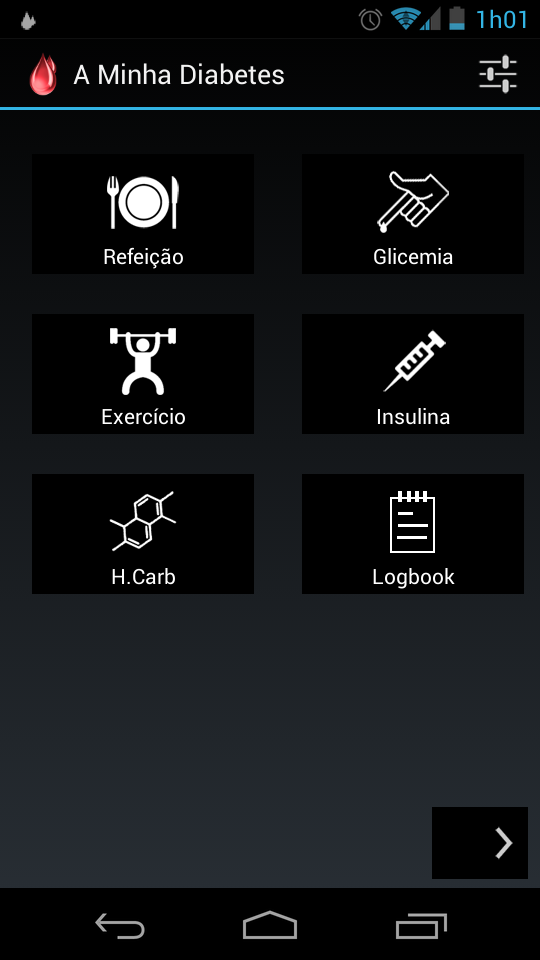
\includegraphics[scale=0.3]{/home/tiago/Tese/Tese/Databases/CSV/Data/ImagensTese/mainmenu.png}
\caption{Menu principal da aplicação MyDiabetes}
\end{figure}

\chapter{Análise de dados}\label{chap:dese}

Neste capítulo será discutido o que foi feito nesta dissertação. Serão abordados requisitos para realizar o trabalho, as decisões tomadas e respetiva explicação e as dificuldades encontradas, que levaram a eventuais alterações aos objetivos inicialmente propostos. Serão ainda mostrados os vários tipos de análises efetuadas aos dados recolhidos, bem como alguns resultados daí obtidos. 

\section{Descrição do estudo}

Para que este estudo pudesse ser feito, o primeiro passo era ter um conjunto de dados de pacientes diabéticos de forma a ser analisado. Este conjunto de dados tinha que ter algumas características específicas para que pudesse ser utilizado da forma pretendida: tinha que ser um conjunto de registos para cada paciente ao longo de algum tempo, sendo que idealmente, no mínimo, cada paciente teria registos correspondentes a quatro semanas. Depois de uma pesquisa, foi possível concluir que não existia, na \textit{web}, qualquer \textit{data set} com estas características.
Para que este estudo pudesse ser feito, era necessário ter um \textit{data set} com os diferentes parâmetros que pudessem ser relevantes, como glicemia, insulina, hidratos de carbono e exercício. 
Como já mencionado, nenhum \textit{data set} existente \textit{on-line} tinha as características desejadas pois só possuíam um registo por pessoa e/ou o seu propósito era a classificação de um paciente como diabético ou não. O único \textit{data set} encontrado que tinha vários registos por pessoa ao longo do tempo tinha o inconveniente de ter apenas dados relativos a glicemias.

Face à falta de dados disponíveis, a solução encontrada foi recolher, de raíz, os dados para a criação do \textit{data set} desejável. Ao podermos construir o nosso próprio \textit{data set} tínhamos a vantagem de podermos recolher as variáveis que queríamos, e portanto, ter um conjunto de dados que torne este trabalho mais eficiente. Por outro lado, visto que a recolha dos dados seria feita através da aplicação MyDiabetes, havia a desvantagem desta ser ainda fechada ao público e, portanto, não ter doentes diabéticos a utilizá-la. Uma outra desvantagem era o tempo que a criação de um \textit{data set} com a variedade e tamanho desejáveis poderia levar. Por variedade e tamanho desejáveis entenda-se dados relativos a cerca de 20 pessoas durante algumas semanas.

Feitas as contas, apesar das desvantagens enunciadas, a solução seria mesmo recolher os dados através da aplicação, sendo que o primeiro passo seria arranjar voluntários. O processo de recolha de dados é descrito na próxima secção.

\section{Recolha de dados}

A recolha de dados foi feita em parceria com o Hospital de S. João, através do seu serviço de endocrinologia. Para tal, foi pedido à comissão de ética autorização para falar com os pacientes diabéticos do hospital e para que estes utilizassem a aplicação, enviando os respetivos registos, pedido esse que foi aceite. Qualquer paciente seria elegível para o projeto desde que tivesse mais de 18 anos e fosse insulino-dependente. 

O Dr. Celestino Neves, médico endocrinologista daquele serviço, serviu de ponte entre a faculdade e o hospital. Nesta primeira fase, o Dr. Celestino dava uma pequena explicação do projeto ao paciente antes, durante ou depois da consulta, sendo que depois re-encaminhava o paciente para nós, investigadores. Esta primeira abordagem do Dr. Celestino era bastante importante uma vez que tornava os pacientes mais recetivos à participação. No nosso encontro com os pacientes, explicávamos o que era o projeto, mostrando no que a aplicação consistia e como funcionava. Depois desta parte, dávamos a conhecer ao paciente os passos seguintes, nomeadamente a integração de um sistema de conselhos baseados no \textit{input} do utilizador. Durante este processo, explicávamos ao paciente a importância de termos dados reais de utilizadores e portanto a importância do envio dos registos, realçando que a longo prazo, os utilizadores seriam os maiores beneficiados, pois poderiam melhorar o seu controlo da glicemia. Os pacientes eram ainda informados que os registos enviados seriam utilizados apenas para fins de investigação e que, caso aceitassem participar no projeto, teriam de assinar um consentimento informado que explicava isso mesmo.

Se os pacientes aceitassem fazer parte do projeto, a aplicação era então instalada nos seus \textit{smartphones} e seria-lhes também dado acesso à aplicação na \textit{Google Play}. Assim, a aplicação passaria a estar sempre disponível para esse utilizador, mesmo que este formatasse ou trocasse o telemóvel, a partir da loja. Outra vantagem deste acesso seria os utilizadores poderem usufruir das atualizações entretanto feitas: sempre que houvesse uma atualização, apareceria o aviso e o utilizador poderia atualizar sem perder os registos já feitos.

Além da aplicação, eram também dadas aos voluntários as credenciais para terem acesso ao \textit{website} do projeto, para onde poderiam exportar os registos efetuados e visualizá-los através de gráficos. As credenciais garantiam assim que apenas os voluntários tinham acesso à parte privada da página, que tem tutoriais e a parte de visualização dos dados.


\subsection{Números e \textit{feedback}}

Este processo era feito duas vezes por semana, que correspondia aos dias de consultas da diabetes, durante aproximadamente três meses. Durante este tempo falámos com várias dezenas de pacientes, sendo que foi possível obter, logo à partida, uma conclusão: a esmagadora maioria dos pacientes com quem falámos estavam bastante recetivos à ideia e concordavam que podia ser uma mais-valia na melhoria da sua qualidade de vida. Muito poucos pacientes tinham a opinião de que a aplicação não teria utilidade, principalmente devido ao facto de estes utilizarem bomba, que torna o processo de controlo da glicemia muito mais reduzido e simples.
Além da idea em si, que foi bastante bem recebida, os utilizadores também deram \textit{feedback} positivo relativamente ao \textit{design} e funcionalidades da aplicação. 

Apesar de todos os pacientes acharem boa ideia ter uma aplicação como esta, nem todos se tornaram voluntários devido a diferentes razões: 1) nem todos os utilizadores tinham \textit{smartphone} e cerca de metade dos pacientes tinha outro sistema operativo que não Android e 2) alguns pacientes com idade mais avançada ou com outros problemas de saúde simplesmente não tinham tempo ou não disponibilidade para participar como voluntário. 
No final deste período tínhamos conseguido a participação de 31 voluntários. Apesar de este número ser suficiente para o que se pretendia, pois inicialmente tinha sido definido como objetivo pelo menos 20 participantes, nem todos os voluntários enviaram, de facto, os registos. 
Dos 31 voluntários apenas 8 enviaram registos pelo menos uma vez e apenas 5 destes enviaram registos relativamente a algumas semanas. Isto foi um dos principais problemas encontrados: para integrar um sistema de aconselhamento baseado nos dados introduzidos numa aplicação para \textit{smartphone} é fundamental saber que tipo de avisos ou conselhos se deve ou não mostrar. Por exemplo, um conselho como "Ajuste a insulina à quantidade de hidratos de carbono ingerida" é algo óbvio e que qualquer paciente diabético sabe, e portanto não seria uma grande mais valia para a alicação. Por outro lado, um aviso como "Hoje é segunda-feira e geralmente à segunda-feira tem valores de glicemia mais elevados" pode ser útil porque possivelmente é um padrão que o paciente não detetou. Neste caso, este conselho poderia fazer o utilizador controlar mais frequentemente a sua glicemia às segundas-feiras e, portanto, normalizar os valores das segundas-feiras a partir daí. 

Esta distinção entre avisos ou conselhos realmente úteis ou descartáveis é importante: se a aplicação mostrar demasiados conselhos intuitivos ou regras "banais" das quais os utilizadores já tenham conhecimento, estes podem acabar por achar que a aplicação não traz benefícios. Pelo contrário, se a aplicação mostrar conselhos baseados em comportamentos errados para cada utilizador, estes podem aperceber-se de que realmente têm esses comportamentos errados e usufruir verdadeiramente deste sistema de aconselhamento. 

Para fazer esta distinção torna-se importante obter a maior quantidade e variedade possível de dados. Imaginemos que temos apenas um \textit{data set} de um paciente com registos de uma semana. Esta quantidade de dados não permite concluir nada sobre eventuais regras descobertas nem sequer permite descobrir vários tipos de regras; tanto a variedade de pacientes como a quantidade de registos serão demasiado reduzidas para tal. 

Da mesma forma, os registos de 5 pacientes, embora seja obviamente mais vantajoso do que o registo de apenas 1 paciente, não é suficiente para esta parte. Uma vez mais, 5 pacientes não oferecem muita quantidade nem variedade em relação a rotinas ou comportamentos errados, que se traduz na variedade de regras produzidas. 

O objetivo da aplicação é gerar os tais conselhos de forma automática e, pensado desta forma, esta parte inicial pode parecer inútil: para quê estar a gerar regras se elas não vão ser utilizadas na aplicação em si? 

Esta questão prende-se, uma vez mais, com a filtragem de regras úteis ou não. Os registos de um único paciente podem gerar, por exemplo, centenas ou até milhares de regras. Obviamente que em milhares de regras muitas vão ser bastante parecidas e a esmagadora maioria vão ser regras que não têm relevância. É possível, por exemplo, que em alguns milhares de regras só se consiga aproveitar 5 ou 6. A importância de ter registos de vários pacientes prende-se com a variedade das regras geradas: dois pacientes podem gerar poucas regras cada um mas essas regras serem diferentes, ou seja, relativas a rotinas ou anomalias com efeitos ou causas diferentes. Esta análise dos dados à procura de regras servirá, então, para construir um conjunto de regras passíveis de ocorrer no dia-a-dia de um diabético que serão então integradas nesta aplicação. Assim, serão apenas detetados padrões e situações que possam ter alguma relevância e conselhos como "Adeque a insulina aos hidratos de carbono" não serão mostrados. Isto porque apesar de ser um bom conselho, também é óbvio e portanto provavelmente será tido como um conselho inútil por parte dos utilizadores. 

Ao ter esta filtragem para mostrar apenas conselhos realmente importantes, não só diminuiremos a quantidade de vezes que algum conselho é mostrado, tornando assim a aplicação menos "chata" para os utilizadores, como também tornam os conselhos mais especiais, ou seja, se um conselho ou aviso é mostrado é porque o utilizador tem de facto algum comportamento errado e que pode ser corrigido.

Neste sentido, a pouca quantidade de voluntários que enviaram registos foi a primeira dificuldade encontrada e que nos fez alterar a estratégia: uma vez que os dados existentes não seriam suficientes para fazer o sistema de aconselhamento de uma forma tão fidedigna quanto desejável, esse objetivo foi posto de lado. Face a estas novas circunstâncias, o objetivo passou a ser analisar os dados existentes das mais variadas formas para ver que tipo de conclusões se consegue obter. Os diferentes tipos de análises feitas vão ser descritos ainda neste capítulo.

Apesar de os dados serem poucos, a parte positiva é que estavam no formato pretendido e portanto o passo seguinte era começar a tratá-los.


\subsection{O \textit{data set}}

Os registos dos utilizadores são armazenados no telemóvel numa base de dados \textit{sqlite}[sqlite] que é depois convertida para um ficheiro csv através de um \textit{script}.[script] O \textit{script} converte cada uma das tabelas num ficheiro csv e depois, os ficheiros csv que interessa manter são copiados para um único ficheiro através do comando \textit{copy}.

Depois de selecionar as variáveis pretendidas e as juntar no mesmo ficheiro, o \textit{data set} fica com a estrutura a seguir apresentada:
 

\begin{table}[H]
\centering

\label{my-label}
\begin{tabular}{|l|l|}
\hline
\textbf{Variável} & \textbf{Tipo} \\ \hline
DateTime          & Integer       \\ \hline
Value\_Carbs      & Integer       \\ \hline
Value\_Glucose    & Integer       \\ \hline
Target\_BG        & Integer       \\ \hline
Value\_Insulin    & Double        \\ \hline
Exercise          & Integer       \\ \hline
\end{tabular}
\caption{My caption}
\end{table}

A variável \textbf{DateTime} diz respeito ao dia e hora exatos de cada registo;
\textbf{Value\textunderscore Carbs} é a quantidade de hidratos de carbono;
\textbf{Value\textunderscore Glucose} é o nível de glicemia à hora do registo;
\textbf{Target\textunderscore BG} é o objetivo de glicemia para a hora do registo, pois o utilizador pode ter diferentes objetivos de glicemia para diferentes períodos do dia. Esta variável é importante para o cálculo da insulina a administrar.
\textbf{Value\textunderscore Insulin} é a quantidade de insulina tomada pelo utilizador à hora do registo;
\textbf{Exercise} corresponde ao exercício feito à hora do registo.\newline

Este \textit{data set} não representa, no entanto, todos os dados enviados pelos utilizadores, pois há alguns dados que não são relevantes para a análise e por isso são descartados. Alguns dos dados descartados são os dados pessoais do utilizador, que incluem, entre outros, nome, idade, peso ou altura; A forma como a aplicação funciona faz com que, a cada registo, sejam registados não só os valores dos parâmetros como outras informações: em cada registo são guardados outros dados como o ID do registo ou a "Tag", que é uma variável opcional que pode associar um registo a um evento. Por exemplo, ao registar uma refeição é possível escolher várias "Tags" como "pequeno-almoço" ou "almoço"; é também guardada uma variável "Note" que permite ao utilizador adicionar uma nota a uma medição. Por exemplo, se o utilizador fizer um registo de exercício, pode adicionar uma nota com "Corrida". Portanto, o registo de cada parâmetro faz com que estas variáveis também sejam guardadas, mesmo que o utilizador não as preencha. O facto de descartarmos estas variáveis não significam que não tenham importância: a variável "Note", por exemplo, pode ser importante se o utilizador quiser adicionar alguma informação extra que ache relevante para depois se lembrar ou até mostrar ao médico. Apenas não são relevantes para este tipo de análise: uma nota sobre uma refeição não pode ser utilizado por um algoritmo. Outras variáveis, como o ID de cada registo, também não são importantes para análise pelo que são descartadas. 

Neste ponto, temos as variáveis com as quais iremos trabalhar, mas que ainda precisam de ser pré-processadas. O pré-processamento do \textit{data set} será descrito de seguida.

\subsection{Pré-processamento dos dados}

Uma parte crucial de \textit{data mining}, ainda antes de aplicar quaisquer técnicas, é a parte de pré-processamento dos dados. Esta parte é composta por várias etapas:

\begin{itemize}
\item Limpeza dos dados
\item Redução dos dados
\item Transformação dos dados
\end{itemize}
 
O pré-processamento dos dados é necessário para tratar inconsistências que possam existir no \textit{data set}. Estas inconsistências podem ser valores em falta ou valores errados. Por exemplo, num \textit{data set} com um campo "Idade", um valor negativo neste campo é um valor errado. Então, para chegar a um estado em que o \textit{data set} esteja pronto a ser utilizado, é preciso percorrer um ou mais dos passos acima mencionados. 

\textbf{Limpeza dos dados} - é o primeiro passo a fazer num conjunto de dados. Neste caso específico, o \textit{data set} vinha com alguns valores em falta ou valores errados. Apesar destes casos serem uma percentagem pequena do total, é importante que sejam resolvidos. Para valores em falta há duas opções: ou remover o registo em que um dos valores falte, ou tentar prever o falor em falta e preenchê-lo. A segunda opção pode ser feita obtendo, por exemplo, a média dessa variável e, em todos os registos com valor em falta, colocar a média. No entanto, para o caso específico da diabetes esta alternativa não parecia a mais viável. Por exemplo, se num dado registo faltar o valor da glicemia, não faz sentido encontrar a média da glicemia para todos os registos e colocar no registo em falta. A glicemia pode oscilar bastante e portanto, estar a preencher um valor em falta com um valor médio da glicemia pode estar a comprometer a veracidade da análise posterior: um registo que até podia ter um valor de hiperglicemia estaria a ser substituído com um valor de glicemia mais normal e portanto, esse registo já não seria uma exceção. Repetindo isto para todos os valores de glicemia em falta, estaria-se a normalizar situações que podiam não ser normais. Posto isto, a alternativa tomada foi a de apagar todos os registos que tivessem valores de glicemia em falta ou valores anormais. Por exemplo, alguns registos tinham valores "0" ou "7", que não são valores realistas para glicemia e portanto trata-se um erro de registo. Assim garante-se que todos os registos tenham valores e que esses valores sejam valores realistas. Esta medida foi tomada apenas para as variáveis necessárias para análise, isto é, para uma análise apenas com a glicemia, as outras variáveis não são tidas em conta e portanto não são limpas. Já para uma análise de procura de regras, como todas as variáveis são utilizadas, todas as variáveis são limpas. 

Isto garante também que as regras geradas não são enviesadas: se quisermos descobrir regras que relacionem os valores de insulina e hidratos de carbono com os valores de glicemia, mas utilizarmos registos que tenham alguns valores de insulina ou hidratos de carbono a zero, então esses registos vão contribuir tanto como os outros para o resultado final, pelo que esse resultado poderá estar adulterado. Limpando um registo inteiro, qualquer que seja o valor da variável em falta ou com um valor errado, garantimos que qualquer resultado obtido numa análise será realista.


\textbf{Redução dos dados} - Num \textit{data set} nem todos os dados têm a mesma relevância: uns são importantes e outros são menos importantes ou até mesmo irrelevantes. É importante perceber quais os dados que não interessa ter, pois assim vamos reduzir a quantidade de regras irrelevantes que são geradas. Por isso mesmo, o segundo passo seria analisar todos os dados recolhidos e perceber quais os que valiam a pena manter e os que se podia remover. Um exemplo que ajuda a perceber melhor este passo é olharmos para os valores de glicose, insulina e hidratos de carbono: na aplicação, cada um destes parâmetros permite registar o valor em si mas também adicionar uma nota para acompanhar o registo. Essa nota poderá ser uma breve descrição feita pelo utilizador aquando de um registo. Existe também um outro atributo chamado "Tag" que permite, por exemplo, associar uma refeição a um período do dia. Se a "Tag" 1 for "pequeno-almoço", então sempre que o utilizador regista o pequeno-almoço, pode escolher essa fase do dia, e esse registo ficará com a "Tag" 1. Como se pode perceber, atributos como "Note" ou "Tag" podem ajudar a perceber o porquê de alguma alteração nos valores de glicose mas não têm qualquer uso para a descoberta de padrões e consequente geração de regras. Portanto, atributos como estes podem ser retirados do \textit{data set} de forma a reduzir a quantidade de informação não relevante. Existem outros atributos que foram retirados por não apresentarem qualquer utilidade para o resultado pretendido, tais como, "Idade", "Nome", "Altura" ou "Sexo". 
No final deste passo, o conjunto de dados é consideravelmente mais pequeno, em termos de quantidade de variáveis, e portanto permite fazer uma análise mais objetiva, com menos informação desinteressante.

\textbf{Transformação dos dados} - Por fim, este passo serve para transformar os valores existentes em valores que possam ser utilizados da forma mais conveniente. Ter uma variável "DateTime" no formato ``AAAA-MM-DD HH:MM''  não é tão útil visto que o dia e hora, que até podem ser variáveis interessantes, estão numa só variável e torna o seu uso mais difícil. Neste caso, seria mais vantajoso separar as duas variáveis e portanto, transformar "DateTime" em "Day" e "Hour". Ainda assim, ter um dia do ano e uma hora específica do dia não é exatamente o formato mais útil, pois são variáveis demasiado específicas e por isso pouco repetidas, ou até nunca repetidas, pelo que não irão contribuir para a descoberta de padrões. Para melhorar este detalhe, podia ainda fazer-se outra alteração: transformar o dia do ano em dias da semana e transformar a hora do dia em período do dia, como "manhã", "noite", ou "tarde". Assim, transformámos a variável "DateTime" em duas variáveis, "Day" e "Period".
Sempre que um utilizador regista uma refeição, com base na glicemia, na glicemia que pretende atingir e nos hidratos de carbono que ingere, é calculada a insulina a tomar. Contudo, o utilizador pode optar por não seguir a dosagem recomendada e tomar mais ou menos. Tendo isto em conta, pode ser importante ver os efeitos que isto provoca e portanto criou-se uma nova variável ``Insulin\textunderscore Difference''. 
A variável ``Insulin\textunderscore Difference'' é calculada com base na fórmula\newline\newline

\begin{lstlisting}[caption=Fórmula para calcular insulina a ser tomada, label=form]
Insulin_Difference = Value_Carbs / RH + ((Value_Glucose - OG)/FS)
\end{lstlisting}


em que ``RH'' é o rácio de hidratos de carbono, ``OG''  é o objetivo de glicemia e ``FS''  é o fator de sensibilidade. Estes valores são diferentes para cada utilizador e cada utilizador pode ter vários objetivos de glicemia por dia. 
Com esta nova variável, se o utilizador optar por tomar uma quantidade de insulina diferente da sugerida com frequência, e isto tiver efeito negativo na glicemia, este padrão será detetado. 

Neste momento o \textit{data set} era composto por 7 variáveis: ``Day'', ``Period'', ``Value\textunderscore Carbs'', ``Value\textunderscore Glucose'', ``Value\textunderscore Insulin'', ``Insulin\textunderscore Difference'' e ``Blood\textunderscore TG''.



Relembrando que ``Day'' e ``Period'' foram transformadas através da variável original, ``DateTime''. A variável ``Day'' foi obtida aplicando a função \textit{weekdays} [weekdays] do \textit{package ``base''} do R. A variável ``Period'' tem como objetivo discretizar a hora do registo: ``Period'' não diz respeito a uma hora mas sim a um intervalo. Assim sendo, ``Period'' tem três valores possíveis:

\begin{itemize}
\item \textbf{1} - Manhã (06:00 - 11:59)
\item \textbf{2} - Tarde (12:00 - 19:59)
\item \textbf{3} - Noite (20:00 - 05:59)
\end{itemize}

o que garante que um dado registo vá pertencer a um dos períodos existentes. Se em vez de usar um intervalo de horas, fossem usadas as horas certas, isso faria com que fosse muito mais difícil encontrar padrões: por exemplo, um registo às 08:30 e outro às 09:30 pertencem ambos ao período 1 mas a horas diferentes. Para que haja um padrão, é necessário que haja repetição de valores. Neste exemplo, se fossem usadas as horas certas os valores seriam diferentes mas usando intervalos de tempo, ambos os registos pertencem ao mesmo período, o da ``Manhã''. Se pensarmos que um dia tem 24 horas e cada hora tem 60 minutos, usando uma variável ``Hora" teríamos 1440 valores possíveis. Por outro lado, usando ``Period'' temos apenas 3 valores diferentes. 

Quanto às variáveis ``Value\textunderscore Glucose'', ``Value\textunderscore Insulin'' e ``Value\textunderscore Carbs'', também tiveram que ser discretizadas, uma vez que se tratavam de variáveis contínuas, ainda que em diferentes intervalos. A glicemia de um paciente diabético pode osclinar entre 50 mg/dL e 300 mg/dL, por exemplo. Já a insulina e os hidratos também podem variar mas os intervalos são mais pequenos, principalmente na insulina. 
Posto isto, a solução foi discretizar estras três variáveis em intervalos, tal como no período do dia. 
Uma solução seria divir em três partes para cada um dos atributos mas visto que se tratam de variáveis importantes, o melhor foi dividir em mais intervalos, nomeadamente 5.
Tome-se o exemplo da glicemia: para pessoas com diabetes, os valores recomendados de glicemia antes das refeições estão entre 70 mg/dL e 130 mg/dL e depois das refeições são entre 90 mg/dL e 160 mg/dL. [levels] Uma vez que esta doença costuma provocar oscilações na glicemia, é comum que os valores estejam no intervalo recomendado mas também estejam acima ou abaixo desse intervalo. Por vezes podem estar muito acima, tratando-se de uma hiperglicemia, ou muito abaixo, no caso de uma hipoglicemia. Sabendo apenas que um valor está acima do recomendado não dá muita informação. Depois de uma refeição, tanto 170 mg/dL como 300 mg/dL são valores acima do intervalo acima mostrado. A diferença é que o primeiro valor é um pouco acima e não é preocupante, enquanto que o segundo valor é muito mais preocupante e requer ação imediata. Isto para mostrar que, ao discretizarmos os valores de glicemia, é importante que o façamos com vários níveis: dizer que um valor está acima do recomendado não chega, é preciso diferenciar o quão acima está. Deste modo, tanto para a glicemia, como insulina e hidratos de carbono, decidiu-se discretizar os valores em cinco níveis:

\begin{itemize}
\item \textbf{1} - Valor muito abaixo do normal e possível hipoglicemia;
\item \textbf{2} - Valor um pouco abaixo do normal;
\item \textbf{3} - Valor normal;
\item \textbf{4} - Valor um pouco acima do normal;
\item \textbf{5} - Valor muito acima do normal e possível hiperglicemia;
\end{itemize}

Estes intervalos não são fixos, variando para cada utilizador. Os extremos são definidos pelo próprio utilizador, ao escolher na aplicação os limites para hipo e hiperglicemia. O valor 3 é definido tendo em conta a média de todas as glicemias do utilizador e os valores 2 e 4 são definidos através do 1º e 3º quartil de todos os valores, respetivamente. Além de ter isto em conta, é preciso também ter em conta os intervalos recomendados em cima definidos. Isto é, se a média dos valores de glicemia de um utilizador for acima do intervalo recomendado, então não fará tanto sentido definir o valor 3 como essa média. No entanto, sempre que a média das glicemias estiver dentro de um intervalo considerado normal, o valor 3 será definido como essa média.

O processo de discretização para os hidratos de carbono e insulina é o mesmo: um valor 5 para hidratos de carbono mostra que o utilizador ingere uma quantidade bastante maior que a recomendada tal como um valor 5 para insulina mostra que o utilizador toma uma dose de insulina muito maior que a recomendada. Naturalmente que um extremo (1 ou 5) em qualquer variável é sempre algo indesejável: consumir demasiados hidratos de carbono pode levar a uma hiperglicemia assim como tomar demasiada insulina pode provocar uma hipoglicemia.

Quanto ao valor da insulina calculada para cada registo, ``Insulin\textunderscore Difference'', o processo é ligeiramente diferente. A insulina é calculada com base na fórmula acima apresentada para calcular a insulina recomendada para cada registo, tendo em conta os valores de glicemia e hidratos de carbono desse mesmo registo. A insulina calculada é então subtraída à insulina tomada pelo utilizador e essa diferença será o valor da variável ``Insulin\textunderscore Difference''. Depois, tal como nas outras variáveis, esta é também dividida em 5 intervalos, que são:

\begin{itemize}
\item \textbf{1} - O valor de insulina tomado é muito menor que o valor calculado
\item \textbf{2} - O valor de insulina tomado é ligeiramente menor que o valor calculado
\item \textbf{3} - O valor de insulina tomado é o calculado
\item \textbf{4} - O valor de insulina tomado é ligeiramente maior que o valor calculado
\item \textbf{5} - O valor de insulina tomado é muito maior que o valor calculado
\end{itemize}

Desta forma será possível encontrar relações, se existirem, entre mudanças no valor da insulina a tomar que possam levar a valores de glicemia indesejados. 


Depois deste processo, o \textit{data set} está num estado em que já pode ser utilizado para algumas análises. Na próxima secção serão mostradas algumas análises básicas de estatística envolvendo os dados referentes a alguns utilizadores. Noutras secções mais à frente, outro tipo de análises serão efetuadas. Algumas dessas análises requerem novas mudanças nos dados, principalmente questões técnicas associadas com algumas funções do R. Essas alterações serão descritas sempre que necessário. De notar as variáveis discretizadas serão utilizadas apenas na parte de associação, pelo que na próxima secção serão feitas análises ainda com os valores exatos de glicemia. Também é importante referir que a varíavel ``Insulin \textunderscore Difference'' é calculada tendo em conta os valores exatos de glicemia e hidratos de carbono, pelo que essa variável é calculada antes da discretização das outras variáveis. 

\section{Análise estatística básica}

Com o \textit{data set} pré-processado, estávamos em condições de começar a utilizá-lo para análise. Antes de começar a aplicar técnicas de \textit{data mining} começou-se por fazer algumas estatísticas com os valores de glicose dos utilizadores. Nas próximas subsecções vamos descrever algumas estatísticas feitas para alguns utilizadores que enviaram registos. Para fazer uma análise minimamente fidedigna é necessário ter uma quantidade considerável de dados pelo que vamos analisar os dados de utilizadores que enviaram registos referentes a quatro ou mais semanas. Começaremos com algumas análises mais simples, fazendo algumas estatísticas que possam permitir observar algumas anormalias nos valores de glicemia. Serão então feitas as diferentes análises para cinco utilizadores de forma totalmente anónima.


\subsection{Média de glicose}

Uma primeira estatística poderia ser simplesmente a média de glicose para um determinado utilizador. Relembrando que o HbA1c é um parâmetro importante para verificar o controlo da diabetes num paciente visto que é possível determinar a média de glicose de algumas semanas ou meses. Portanto, de uma maneira mais ou menos semelhante, a média de glicose de um determinado paciente dá para ter uma idea do quão bem esse paciente controla a glicemia. Apresentam-se de seguida as médias de glicose para os cinco utilizadores:

\begin{itemize}
\item \textbf{Utilizador 1} - 119 mg/dL
\item \textbf{Utilizador 2} - 150 mg/dL
\item \textbf{Utilizador 3} - 170 mg/dL
\item \textbf{Utilizador 4} - 144 mg/dL
\item \textbf{Utilizador 5} - 154 mg/dL

\end{itemize}

Como mencionado anteriormente, estas médias pertencem a diferentes utilizadores e dizem respeito a registos durante pelo menos quatro semanas, e portanto, são um indicador geral do controlo da glicemia por parte de cada utilizador. Pode perceber-se que alguns utilizadores têm uma média com um valor mais normal que outros o que pode ser um indicador de um bom controlo. No entanto, isto não é necessariamente verdade. Um bom controlo da glicemia passa não só por manter os valores em intervalos normais mas também em prevenir grandes oscilações. Neste caso, uma média de glicemia de 119 mg/dL pode parecer melhor que uma média de glicemia de 170 mg/dL mas pode não ser: o primeiro utilizador pode ter 2 registos em que um seja 60 mg/dL e outro seja 180 mg/dL, o que dá uma média de 120 mg/dL; por outro lado, o terceiro utilizador pode ter ambos os valores a 170 mg/dL. Ou seja, embora a média de glicemia do primeiro utilizador seja mais baixa, não significa que os valores sejam estáveis, tal como no terceiro utilizador não significa que os valores não sejam estáveis. Medir apenas a média da glicemia é uma análise demasiado vaga: pode ser um indicativo de um bom ou mau controlo da glicemia mas não permite ter certezas. Torna-se portanto necessário fazer uma análise mais aprofundada.



\subsection{Média de glicose por dia}

Uma forma mais detalhada de tentar perceber alguns hábitos dos utilizadores é verificar como é que a sua glicemia oscila durante a semana. Tal pode ser feito obtendo a média de glicose para cada dia. Assim, é possível saber, por exemplo, quais os dias em que a glicemia é mais elevada ou mais baixa, sem esquecer que se trata de uma média, e que por isso não é possível ter conhecimento sobre eventuais hipo ou hiperglicemias. Ainda assim, ao saber a média de glicemia por cada dia, será possível avisar o utilizador de quais os dias a ter em atenção, isto é, se a segunda-feira for um dia com uma média elevada de glicemia, então o utilizador pode ser avisado deste facto para tomar as medidas necessárias ou, pelo menos, aumentar o controlo da glicemia neste dia. Portanto, embora este tipo de estatística não permita descobrir situações em particular, pode ainda assim ser útil. Eis os valores médios de glicemia para os utilizadores:\newline

\textbf{Utilizador 1}

\begin{itemize}[noitemsep]
\item \textbf{Domingo}: 132 mg/dL
\item \textbf{Segunda}: 117 mg/dL
\item \textbf{Terça}: 119 mg/dL
\item \textbf{Quarta}: 127 mg/dL
\item \textbf{Quinta}: 110 mg/dL
\item \textbf{Sexta}: 110 mg/dL
\item \textbf{Sábado}: 115 mg/dL
\end{itemize}


\textbf{Utilizador 2}

\begin{itemize}[noitemsep]
\item \textbf{Domingo}: 161 mg/dL
\item \textbf{Segunda}: 131 mg/dL
\item \textbf{Terça}: 154 mg/dL
\item \textbf{Quarta}: 156 mg/dL
\item \textbf{Quinta}: 149 mg/dL
\item \textbf{Sexta}: 14 8mg/dL
\item \textbf{Sábado}: 165 mg/dL
\end{itemize}

\textbf{Utilizador 3}

\begin{itemize}[noitemsep]
\item \textbf{Domingo}: 182 mg/dL
\item \textbf{Segunda}: 162 mg/dL
\item \textbf{Terça}: 189 mg/dL
\item \textbf{Quarta}: 166 mg/dL
\item \textbf{Quinta}: 181 mg/dL
\item \textbf{Sexta}: 163 mg/dL
\item \textbf{Sábado}: 146 mg/dL
\end{itemize}


\textbf{Utilizador 4}

\begin{itemize}[noitemsep]
\item \textbf{Domingo}: 149 mg/dL
\item \textbf{Segunda}: 170 mg/dL
\item \textbf{Terça}: 165 mg/dL
\item \textbf{Quarta}: 114 mg/dL
\item \textbf{Quinta}: 142 mg/dL
\item \textbf{Sexta}: 131 mg/dL
\item \textbf{Sábado}: 136 mg/dL
\end{itemize}


\textbf{Utilizador 5}

\begin{itemize}[noitemsep]
\item \textbf{Domingo}: 182 mg/dL
\item \textbf{Segunda}: 153 mg/dL
\item \textbf{Terça}: 154 mg/dL
\item \textbf{Quarta}: 150 mg/dL
\item \textbf{Quinta}: 170 mg/dL
\item \textbf{Sexta}: 140 mg/dL
\item \textbf{Sábado}: Não registou
\end{itemize}

Com uma análise deste tipo, embora não se possam tirar conclusões sobre a forma como a glicemia varia, podemos começar a ter algum conhecimento sobre o que podem ser rotinas dos utilizadores. Por exemplo, para 4 dos 5 utilizadores acima mostrados, o dia em que o valor médio de glicemia é mais elevado é aos Domingos. Normalmente ao fim-de-semana as pessoas tendem a ter um estilo de vida mais sedentário e relaxado, o que por sua vez pode levar a um controlo menos apertado da glicemia; mesmo que o controlo não seja afetado ao fim-de-semana, pode haver quem não tenha tanto cuidado com a comida, cometendo alguns excessos; pode até apenas ser o facto de as pessoas estarem menos \textit{stressadas} ao fim-de-semana. Mais importante de saber o porquê de estes valores serem mais elevados ao Domingo, o importante é o conhecimento de que isto acontece. É impossível adivinhar o porquê de os valores serem tendencialmente maiores a um determinado dia, apenas sabendo a média dos valores, mas o simples facto de descobrir esse facto e de alertar um utilizador para o mesmo, pode fazer com que ele próprio se aperceba o que faz de diferente e que provoce a alteração, podendo assim corrigi-la. 
No contexto da aplicação, uma simples estatística como esta acima mostrada, podia fazer aparecer um aviso, alertando o utilizador que a um determinado dia da semana, os valores de glicemia são, em geral, mais altos. Este processo seria automático: a aplicação calcularia o valor da média para cada dia e mostraria um aviso sempre que este valor fosse mais alto que o desejado. Imaginemos que o utilizador 3 definiu o limite de hiperglicemia como 180. A aplicação ao calcular a média de glicemia para cada dia verificava que em três dias diferentes da semana os valores costumam ser acima desse limite e portanto lançaria um aviso.\newline

Pode concluir-se que este tipo de estatística é mais vantajoso que o primeiro, porque pode ajudar a identificar dias em que os valores são mais anormais. Uma vez mais, a média de glicemia não permite saber cada valor exatado de cada medição, pelo que ainda não é possível verificar se os valores são estáveis ou oscilatórios. Ainda assim, se a média de um determinado dia é próxima ou até superior ao limite de hiperglicemia definido pelo utilizador, permite saber que há uma grande probabilidade de nesse dia o utilizador ter tido valores acima do limite.

\subsection{Média de glicose por período do dia}

Como já vimos, pode ser útil saber os valores médios de glicemia para cada dia da semana, que nos permite saber que, por exemplo, o Domingo é um dia com valores tendencialmente mais elevados. Mas apenas isso não nos dá qualquer tipo de informação sobre a variação dos valores ao longo do dia, o que também seria útil. Se um utilizador tiver o conhecimento de que tem valores mais elevados à tarde do que no resto do dia, se calhar percebe que o tipo de almoço que normalmente faz pode não ser o mais indicado. Obviamente que isto é só um exemplo, mas o facto é que saber como varia a glicemia durante o dia pode ajudar os utilizadores a perceber eventuais hábitos errados. 
Tendo isto em conta, para a próxima estatística dividiu-se o dia em três partes, como já explicado:

\begin{itemize}
\item Manhã: 06:00 - 11:59;
\item Tarde: 12:00 - 19:59;
\item Noite: 20:00 - 05:59;
\end{itemize}

Os valores médios para cada utilizador em cada fase do dia são:\newline

\textbf{Utilizador 1}

\begin{itemize}
\item Manhã: 112 mg/dL
\item Tarde: 117 mg/dL
\item Noite: 128 mg/dL
\end{itemize}

\textbf{Utilizador 2}

\begin{itemize}
\item Manhã: 160 mg/dL
\item Tarde: 151 mg/dL
\item Noite: 138 mg/dL
\end{itemize}

\textbf{Utilizador 3}

\begin{itemize}
\item Manhã: 162 mg/dL
\item Tarde: 141 mg/dL
\item Noite: 199 mg/dL
\end{itemize}

\textbf{Utilizador 4}

\begin{itemize}
\item Manhã: 158 mg/dL
\item Tarde: 134 mg/dL
\item Noite: 146 mg/dL
\end{itemize}

\textbf{Utilizador 5}

\begin{itemize}
\item Manhã: 154 mg/dL
\item Tarde: 157 mg/dL
\item Noite: 153 mg/dL
\end{itemize}

Este tipo de análise já permite ter uma ideia mais concreta das oscilações da glicemia para cada utilizador ao longo do dia. É possível verificar que alguns utilizadores conseguem manter os níveis de glicemia mais ou menos estáveis, como os utilizadores 1 e 5. É possível observar algumas oscilações mais acentuadas em alguns utilizadores: o utilizador 1 por exemplo, embora consiga manter sempre os níveis de glicemia num intervalo considerado normal, tem tendência para ter valores ligeiramente mais elevados à noite. Isto pode ser devido a menos atividade durante a noite, que normalmente é usada para relaxar. Pode ser também por não adequar a insulina em relação ao jantar, por exemplo. Já no utilizador 2 acontece precisamente o contrário: tem valores mais elevados pela manhã, que vão diminuindo ao longo do dia. Os valores altos pela manhã podem indicar que o utilizador ingere alimentos antes de ir para a cama ou que não adequa a insulina depois do jantar, por exemplo. Uma vez mais, neste tipo de estatística é mais importante detetar comportamentos anormais do que os explicar. 
Quanto ao utilizador 3 é aquele que, pelo que se pode observar apenas com estes dados, apresenta mais oscilações. Começa o dia com valores ligeiramente elevados, pelo que os consegue baixar um bocado durante o dia até que voltam a subir bastante durante a noite. Isto pode não acontecer todos os dias mas geralmente é o que acontece. O aviso nesta situação seria importante para que o utilizador tentasse evitar hiperglicemias durante a noite.

É natural que os valores de glicemia oscilem durante o dia por vários fatores: o \textit{stress} do trabalho pode causar aumento no nível de glicose no sangue. Por outro lado, o esforço físico durante o dia, quando existente, pode provocar o contrário. Mesmo sem fatores externos, por vezes há situações que levam a glicemia a variar de forma natural. Uma dessas situações é conhecida por \textit{dawn phenomenon}, que causa o aumento da glicose no sangue durante a noite, devido a hormonas que o corpo produz nesse período. Isso faz com que o utilizador tenha valores mais altos de manhã. Este pode até ser o motivo para que três utilizadores tenham valores mais elevados de manhã do que nos outros períodos do dia, tal como os motivos anteriores. Independentemente do motivo, a consciência de que isto acontece é o primeiro passo para corrigir a situação.\newline



Na próxima subsecção vamos fazer uma análise ainda mais detalhada, mostrando os níveis de glicemia ao longo do dia e por cada dia da semana. Como já mencionado, apesar de a média de glicemia ser um bom indicativo do controlo da mesma, é mais útil ter valores exatos que permitem ver se, de facto, há oscilações e o quão grandes são essas variações.

\subsection{Glicose por hora do dia}

Os valores de glicose exatos, ao contrário da média, permitem perceber se há variações ou estabilidade na glicemia. Numa primeira análise mostraremos os valores de glicose por hora para todos os dias e posteriormente para cada dia da semana. Desta forma será possível saber a que horas do dia, e em que dias, é que o utilizador geralmente tem mais hiper ou hipoglicemias.\newpage

\textbf{Utilizador 1}

\begin{figure}[H]
\centering
\includegraphics[scale=0.8]{/home/tiago/Tese/Tese/Databases/CSV/Data/ImagensTese/Utilizador1/Horas.png}
\caption{Glicemia por horas do utilizador 1}
\end{figure}

Como se pode perceber pelo gráfico, a esmagadora maioria dos registos são feitos entre as 08:00 e as 24:00, sendo que neste intervalo, grande parte dos registos são feitos estão divididos em três momentos, provavelmente na hora das refeições. A linha vermelha representa o limite mínimo desejável e a linha azul o máximo desejável. Estas linhas correspondem a hipo e hiperglicemia, respetivamente, e foram definidas pelo utilizador, sendo que o limite para hipoglicemia é 70 e para hiperglicemia é 180. Ao analisar o gráfico percebe-se imediatamente que quase todos os valores se encontram entre estes dois valores, o que é desejável, visto que é o intervalo definido como "normal" pelo utilizador. Percebe-se também que há algumas hiperglicemias, sendo que todas elas ocorrem entre o início da tarde e o início da madrugada. Obviamente que isto não significa que durante a madrugada não hajam valores elevados, apenas não são registados. 


\textbf{Utilizador 2}

\begin{figure}[H]
\centering
\includegraphics[scale=0.8]{/home/tiago/Tese/Tese/Databases/CSV/Data/ImagensTese/Utilizador2/Horas.png}
\caption{Glicemia por horas do utilizador 2}
\end{figure}

Ao analisar o gráfico do utilizador 2 percebe-se um dos problemas anteriormente mencionados: as médias podem ser um bom indicador geral mas também podem não o ser. E neste caso não é: a média de glicemia do utilizador 2 é de 150 mg/dL o que poderia levar a pensar que este utilizador tinha valores mais ou menos estáveis. No entanto, observando o gráfico, verifica-se que não é o que acontece: os valores oscilam entre extremos muito separados, havendo valores acima de 300 e outros abaixo de 50. Neste caso os limites definidos pelo utilizador foram de 70 para hipoglicemia e de 150 para hiperglicemia. Também é possível observar que cerca de metade dos registos efetuados encontram-se fora dos intervalos estabelecidos, o que leva a pensar que estes limites escolhidos não foram os mais corretos e talvez tenham de ser adaptados. De qualquer das formas, as medições são feitas mais frequentemente de manhã cedo e ao início da tarde, presumivelmente à hora de pequeno-almoço e almoço. 


\textbf{Utilizador 3}

\begin{figure}[H]
\centering
\includegraphics[scale=0.8]{/home/tiago/Tese/Tese/Databases/CSV/Data/ImagensTese/Utilizador3/Horas.png}
\caption{Glicemia por horas do utilizador 3}
\end{figure}

Ao observar a figura, percebe-se que os valores oscilam bastante, havendo alguns valores próximos de 50 mg/dL e outros próximos de 300 mg/dL. Os limites definidos pelo utilizador foram de 60 mg/dL para hipoglicemia e 180 mg/dL para hiperglicemia. No gráfico do utilizador anterior, haviam vários períodos do dia com hiperglicemia mas estas eram, aproximadamente, em igual número à quantidade de valores normais, isto é, pelo gráfico do utilizador 2, observa-se que no geral, para um determinado período, a quantidade de valores normais ou demasiado elevados são mais ou menos iguais. Por outro lado, neste gráfico observa-se o contrário: há períodos que notoriamente tem mais hiperglicemias que valores normais e outros períodos com mais valores normais que hiperglicemias. 
Por exemplo, entre as 07:00 e as 10:00, que será o período do pequeno-almoço ou imediatamente depois, verifica-se que a quantidade de valores altos e valores normais são parecidas. Já no período imediatamente a seguir à hora de almoço, há poucas hiperglicemias em relação à quantidade de registos feitos. Por último, à hora de jantar ou logo a seguir, a quantidade de hiperglicemias é bastante alta em relação à quantidade das medições. Isto pode ser uma consequência da rotina do utilizador. Por exemplo, se o utilizador jantar e logo a seguir descansar, pode causar esta subida. Por outro lado, e olhando para o gráfico, uma solução poderia ser algum tipo de exercício leve depois do jantar, como uma caminhada, para conseguir baixar um pouco os valores. Outra alternativa seria ajustar a insulina depois do jantar. 
De qualquer das formas, com este tipo de análise, não se consegue descobrir qual a causa para estes valores anormais, pelo que sem um tipo de análise mais profunda, cabe ao utilizador perceber o porquê de isto acontecer.



\textbf{Utilizador 4}

\begin{figure}[H]
\centering
\includegraphics[scale=0.8]{/home/tiago/Tese/Tese/Databases/CSV/Data/ImagensTese/Utilizador4/Horas.png}
\caption{Glicemia por horas do utilizador 4}
\end{figure}

O utilizador 4 definiu como 60 mg/dL o limite para hipoglicemia e 150 mg/dL o limite para hiperglicemia. Tal como já aconteceu com outros utilizadores, os valores de hiperglicemia são abundantes o que pode levar a crer que o limite para hiperglicemia é demasiado baixo e poderia ser ajustado. O utilizador 3 tem geralmente hiperglicemias depois das três refeições o que significa que talvez a insulina devesse ser ajustada. Verifica-se também a presença de alguns valores demasiado altos por volta da meia noite seguidos por valores demasiados baixos durante a madrugada. 


\textbf{Utilizador 5}

\begin{figure}[H]
\centering
\includegraphics[scale=0.8]{/home/tiago/Tese/Tese/Databases/CSV/Data/ImagensTese/Utilizador5/Horas.png}
\caption{Glicemia por horas do utilizador 5}
\end{figure}


Tal como no utilizador passado, neste utilizador, apenas observando o gráfico não se consegue obter conclusões, isto porque não há nenhum período do dia que se destaque dos outros. O utilizador definiu um limite para hipoglicemia de 70 mg/dL e não definiu um limite para hiperglicemia, pelo que o limite utilizado foi 180 mg/dL. Conseguem-se observar alguns períodos com tendência para hiperglicemia, nomeadamente de manhã, ao início da tarde e a meio da tarde. Neste utilizador não é possível concluir nada apenas com esta análise.\newline

Pelos gráficos observados de todos os utilizadores, verifica-se que em todos eles há hiperglicemias, embora nuns notoriamente mais que noutros. Embora não se consigam descobrir padrões ou detetar anomalias apenas com uma análise deste tipo, fica visível a necessidade de um melhor controlo da glicemia por parte de quase todos os utilizadores, que pode ser conseguida através de um uso de uma aplicação de registo, tal como a MyDiabetes. Embora na análise feita nesta subsecção se consigam descobrir mais detalhes do que na subsecção anterior, ainda não é descoberto o suficiente. Desta forma vamos aprofundar ainda mais e fazer uma análise por dia e por hora para cada utilizador.

\subsection{Glicose por hora e por dia}

Nas últimas subsecções fizemos uma análise que nos permite saber que, por exemplo, um determinado utilizador tem tendencialmente valores de glicemia mais elevados à terça-feira ou que um outro utilizador normalmente tem valores de glicose no sangue mais elevados à noite. Mas estas duas conclusões são independentes: saber que os valores são mais altos à terça-feira não nos permite saber como é que os valores variam durante a terça-feira ou saber que os valores são mais altos à noite não nos permite saber em que noites da semana é que os valores são de facto mais elevados. Face a este problema, fez-se uma análise ainda mais detalhada que as anteriores e relacionámos estas duas variáveis, dia da semana e período do dia, para tentar perceber de que forma é que a glicose varia durante o dia, para cada dia da semana. De seguida apresentaremos os gráficos para os cinco utilizadores. 

\textbf{Utilizador 1}

\begin{figure}[H]
\centering
\includegraphics[scale=0.8]{/home/tiago/Tese/Tese/Databases/CSV/Data/ImagensTese/Utilizador1/Dias.png}
\caption{Glicemia por horas do utilizador 1}
\end{figure}

\begin{figure}[H]
\centering
\includegraphics[scale=0.8]{/home/tiago/Tese/Tese/Databases/CSV/Data/ImagensTese/Utilizador1/Dias2.png}
\caption{Glicemia por horas do utilizador 1}
\end{figure}

Analisando as figuras em cima, nota-se que o utilizador mantém grande parte das vezes os valores de glicemia dentro dos intervalos normais todos os dias. No entanto, nota-se claramente que o Domingo tem mais hiperglicemias que os outros dias todos e que estas ocorrem ao final da tarde ou início da noite. Embora as estatísticas anteriores sobre este utilizador mostrem que de facto o Domingo é o dia com a média de glicemia mais elevada e que a noite é o período com média de glicemia mais elevada, tal não significa necessariamente que estas duas médias fossem verdade sempre. Ou seja, nada garantia que ao Domingo a glicemia também fosse mais elevada à noite. Contudo, com esta análise pode perceber-se que de facto isso acontece. Nos outros dias verifica-se que há um ou outro caso de hiperglicemias ou hipoglicemias mas em muito pouca quantidade. Uma análise que utilize os outros parâmetros como insulina ou hidratos de carbono talvez ajude a perceber o porquê de o Domingo ser um dia com valores de glicemia mais altos. 

\textbf{Utilizador 2}

\begin{figure}[H]
\centering
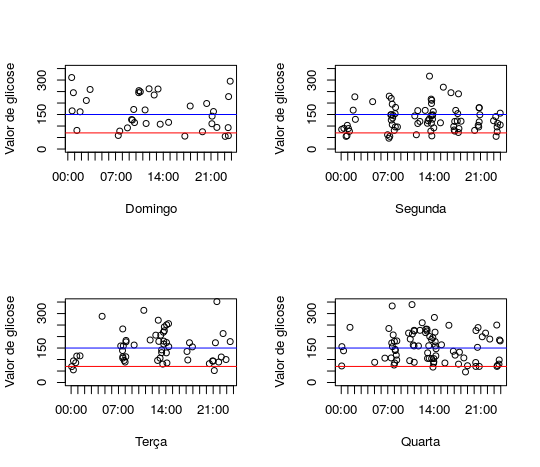
\includegraphics[scale=0.8]{/home/tiago/Tese/Tese/Databases/CSV/Data/ImagensTese/Utilizador2/Days.png}
\caption{Glicemia por horas do utilizador 2}
\end{figure}

\begin{figure}[H]
\centering
\includegraphics[scale=0.8]{/home/tiago/Tese/Tese/Databases/CSV/Data/ImagensTese/Utilizador2/Dias2.png}
\caption{Glicemia por horas do utilizador 2}
\end{figure}

Observando as figuras verifica-se que o utilizador apresenta hiperglicemias todos os dias, maioritariamente durante a tarde. Ao Domingo apresenta menos hiperglicemias porque também tem menos registos. No resto dos dias apresenta uma distribuição semelhante entre valores normais e valores acima do limite de hiperglicemia, isto é, há mais ou menos quantidade de valores normais e valores demasiado altos. Contudo, ao Sábado o número de hiperglicemias é bastante maior em relação ao número de valores no intervalo normal.



\textbf{Utilizador 3}

\begin{figure}[H]
\centering
\includegraphics[scale=0.8]{/home/tiago/Tese/Tese/Databases/CSV/Data/ImagensTese/Utilizador3/Dias.png}
\caption{Glicemia por horas do utilizador 3}
\end{figure}

\begin{figure}[H]
\centering
\includegraphics[scale=0.8]{/home/tiago/Tese/Tese/Databases/CSV/Data/ImagensTese/Utilizador3/Dias2.png}
\caption{Glicemia por horas do utilizador 3}
\end{figure}


Neste utilizador é possível ver um padrão: tem tendência para ter hiperglicemias de manhã e ao fim da tarde ou início da noite. Uma vez mais, a causa pode estar relacionado com o trabalho, por exemplo, que pode ser mais desgastante à tarde, daí fazer com que os valores não subam tanto. Esta teoria seria ainda suportada pelo gráfico de Sábado, que mostra algumas hiperglicemias também a meio da tarde, o que faria sentido se de facto a causa dos valores durante a semana fosse o trabalho. 

\textbf{Utilizador 4}

\begin{figure}[H]
\centering
\includegraphics[scale=0.8]{/home/tiago/Tese/Tese/Databases/CSV/Data/ImagensTese/Utilizador4/Dias.png}
\caption{Glicemia por horas do utilizador 4}
\end{figure}

\begin{figure}[H]
\centering
\includegraphics[scale=0.8]{/home/tiago/Tese/Tese/Databases/CSV/Data/ImagensTese/Utilizador4/Dias2.png}
\caption{Glicemia por horas do utilizador 4}
\end{figure}


Observando as figuras em cima, é possível observar que em todos os dias ocorrem hiperglicemias mas há três dias que se destacam: Domingo, Segunda e Terça, pois têm mais hiperglicemias em comparação com valores normais que o resto dos dias. Verifica-se também que os valores mais altos ocorrem de manhã ou ao início da noite, sendo que apenas em dois dias há mais que uma hiperglicemia a meio da tarde, o que pode significar que o utilizador possa fazer algo de diferente nestes dois dias, embora sem qualquer tipo de certeza. 
Em vários dias da semana notam-se alguns valores muito próximos ou até abaixo do limite de hipoglicemia sendo notórios dois períodos em que eles são mais frequentes: durante a madrugada e perto da hora de almoço. Isto pode significar que o utilizador come nada antes de ir dormir, para o primeiro caso, e para o segundo caso pode significar que o utilizador não come nada entre o pequeno-almoço e o almoço, e que talvez devesse comer alguma coisa. 


\textbf{Utilizador 5}

\begin{figure}[H]
\centering
\includegraphics[scale=0.8]{/home/tiago/Tese/Tese/Databases/CSV/Data/ImagensTese/Utilizador5/Dias.png}
\caption{Glicemia por horas do utilizador 5}
\end{figure}

Para este utilizador mostramos apenas gráficos referentes a três dias já que os outros não têm registos suficientes.



\section{Regras de associação}

Para esta análise as funções que o R oferece não são suficientes pelo que foi necessário instalar um \textit{package} adicional, \textit{arules}, que oferece uma vasta quantidade de funções direcionadas para regras de associação. Ao contrário das secções anteriores, nesta secção usam-se os vários parâmatros com os seus valores já discretizados, para que o algoritmo utilizado seja mais eficiente. O processo de de procura de regras de associação é de fácil compreensão: o algoritmo vai percorrer o \textit{data set} e analisar cada ``transação'', que corresponde a cada linha do ficheiro csv. Dependendo da confiança e suporte escolhidos, vai gerar algumas regras que conseguir encontrar e que respeitem os limites escolhidos. As regras geradas podem ser de qualquer tipo, isto é, o consequente pode ser qualquer uma das variáveis analisadas, sendo que neste caso interessa-nos descobrir regras com a variável ``Value\textunderscore Glucose'' como consequente, ou seja, no lado direito. Contudo, o \textit{data set} ainda não está estruturado da melhor forma para a criação das regras. 
Da forma que o \textit{data set} está feito, cada linha corresponde ao mesmo momento, ou seja, se uma linha tiver um valor de glicemia, hidratos de carbono e insulina, tudo isso corresponde a um registo feito à mesma hora. O mesmo acontece para o exercício. O tipo de conclusões que se pretende obter é de que forma estes parâmetros causam algum impacto no valor de glicemia, como por exemplo, descobrir de que forma o exercício vai alterar a quantidade de glucose no sangue ou de que forma a insulina tomada ou os hidratos de carbono vão fazer alterar este valor. Se todos esses parâmetros forem registados à mesma hora, não se consegue concluir nada: uma vez que o algoritmo Apriori vai analisar linha a linha de forma independente, no formato atual, o valor de glicemia só vai ser comparado com o valor de insulina e de hidratos de carbono registados ao mesmo tempo. No entanto, o importante é saber como é que a quantidade de hidratos de carbono ingerida e a insulina tomada vão afetar a glicemia no espaço de tempo a seguir, e não no mesmo espaço de tempo. Ou seja, como é que os valores de hidratos e de insulina num registo, vão afetar a glicemia no registo seguinte. A questão é que o valor de glicemia do registo seguinte vai pertencer a outra linha do csv e portanto não vai ser tido em conta para os valores de outra linha. Posto isto, a solução foi alterar a estrutura do ficheiro para que cada linha passe a ter o valor de glicemia seguinte, e não o atual. Assim, imaginando que a variável ``Value\textunderscore Glucose'' passe a chamar-se ``Next\textunderscore Glucose'', é possível ter uma regra como

\begin{lstlisting}
Se Value_Carbs==5 entao Next_Glucose==5
\end{lstlisting} 

ou seja, descobrir um padrão em que quando o utilizador ingere demasiados hidratos de carbono, então o valor seguinte de glicemia será demasiado elevado, mais precisamente uma hiperglicemia. Se esta alteração não fosse feita, as regras descobertas apenas dariam relações entre valores registados à mesma hora o que não tem qualquer utilidade. Embora este não seja o único tipo de regras a descobrir, certamente que é um dos tipos de conselhos que podem levar um utilizador a conseguir controlar a diabetes de forma mais eficiente. Convém relembrar que se uma regra é descoberta, é porque essa ação ocorre várias vezes, ou seja, trata-se de um padrão. Ao informar o utilizador de que este padrão existe, e que tem uma influência negativa nos seus valores de glicemia, o utilizador pode tomar a ação que achar mais apropriada de forma a evitar que aconteça. Na presença de uma regra como esta, a aplicação poderia mostrar um aviso quando o utilizador fosse fazer um registo de refeição e metesse um valor elevado de hidratos de carbono, em que o aviso poderia ser, por exemplo, ``Meteu um valor de hidratos de carbono elevado e, quando faz isso, normalmente tende a ter uma eventual hiperglicemia algum tempo depois da refeição''.

Uma vez alterados os \textit{data sets} de cada utilizador, faltava ainda converter todas as variáveis para \textit{factor}. \textit{Factor} é um tipo em R que toma apenas um número limitado de valores diferentes; variáveis do tipo \textit{factor} são também chamadas de variáveis categóricas. Esta conversão é necessária para as variáveis poderem ser utilizadas no algoritmo de associação. Ainda assim, a fase de discretização feita na secção 5.2 é também necessária. Sem a discretização, as variáveis podem ser utilizadas pelo apriori desde que sejam do tipo \textit{factor} mas as regras geradas não são utilizáveis. Por exemplo, uma regra gerada sem fazer discretização das variáveis é

\begin{lstlisting}
{Value_Glucose=140,Value_Insulin=140} => {Value_Carbs=140}
\end{lstlisting}

que serve para ilustrar a ineficácia deste algoritmo para valores não discretizados. Feito então o passo de conversão das variáveis para \textit{factors}, o \textit{data set} está pronto a ser utilizado pelo apriori. De seguida apresentaremos algumas das regras mais relevantes descobertas para cada utilizador e verificaremos também se essas regras estão em concordância com os gráficos obtidos na secção anterior. Todas as regras terão uma confiança mínima de 60\%.
Para cada utilizador interessa-nos descobrir regras que levem a alterações do valor de glicemia, sendo que o valor normal, tal como definido na secção 5.1, é 3. Portanto, interessa descobrir regras em que o valor de glicose seja 1 ou 2 para valores baixos e 4 ou 5 para valores altos.

O algoritmo \textit{apriori} vai analisar linha a linha dos dados e tentar descobrir relações entre as variáveis. Para obter as regras cujo consequente diga respeito aos valores anormais de glicemias, é preciso filtrar as regras geradas. Neste caso, vamos filtrar o conjunto de regras de forma a mostrar apenas regras com ``Next\textunderscore Glucose'' com valores 1, 2, 4 ou 5. 

Para todos os utilizadores definimos uma confiança mínima de 0.6 e um suporte mínimo de 0.01. O suporte tem que ser bastante baixo uma vez que vamos aplicar o algoritmo num \textit{data set} pequeno. Isto porque estamos à procura de padrões que, embora recorrentes, vão ser uma minoria dos dados. Naturalmente que num \textit{data set} com milhares de linhas esses padrões são mais óbvios, ou seja, mais frequentes, e portanto um suporte mais alto seja suficiente para encontrar. Por outro lado, para \textit{data sets} com dezenas ou poucas centenas de linhas, os padrões não são tão explícitos pelo que é necessário um suporte mais baixo para descobrir regras. Usar um suporte demasiado baixo pode fazer com que sejam descobertas regras que sejam um caso pontual, pelo que convém não usar um suporte demasiado baixo. Assim, foi escolhido o valor 0.01 que é um valor baixo mas não demasiado. 

Para a confiança foi escolhido o valor mínimo de 0.6 o que significa que, para cada regra, se o antecedente acontece, então o consequente irá acontecer com 60\% de probabilidade, o que confere alguma segurança às regras. As regras que cumpram estes dois requisitos são chamadas de regras fortes.


No R, o comando para a geração de regras através do algoritmo \textit{apriori} é

\begin{lstlisting}
rules <- apriori(dataset, parameter=list(confidence=0.6, support=0.01))
\end{lstlisting}

em que ``dataset'' é o ficheiro a ser analisado com os parâmetros confiança e suporte definidos com os valores já mencionados. Para mostrar apenas as regras com o valor de glicose pretendido, como por exemplo 5, o comando é

\begin{lstlisting}
rules.sub <- subset(rules, subset = rhs %in% "Next_Glucose=5")
\end{lstlisting}

que gerará então um subconjunto de regras em que o consequente será ``Next\textunderscore Glucose=5''.

Existe um \textit{package} chamado \textit{arulesViz} que é uma ferramenta para visualizar as regras geradas. Este \textit{package} permite, por exemplo, ordenar as regras geradas por confiança ou \textit{lift} e assim filtrar quais as regras potencialmente mais úteis. Isto é feito de forma interativa: no gráfico é possível selecionar uma região com regras e todas as regras existentes nessa região serão mostradas.
De seguida, apresentaremos algumas regras geradas para cada utilizador.

\textbf{Utilizador 1}

Para o utilizador foram geradas 1239 regras. Obviamente que se torna impossível de analisar todas as regras individualmente, pelo que o primeiro passo será então aplicar um filtro, de forma a ficar apenas com valores anormais de glicemia no consequente. Após este filtro, o conjunto de regras diminui bastante, para 25. Com o comando

\begin{lstlisting}
plot(rules.sub, method=NULL, measure="support", shading = "lift", interactive = TRUE, data = NULL, control = NULL)
\end{lstlisting}

obtém-se o gráfico

\begin{figure}[H]
\centering
\includegraphics[width=75mm, height=75mm]{/home/tiago/Tese/Tese/Databases/CSV/Data/ImagensTese/Utilizador1/Regras.pdf}
\caption{Glicemia por horas do utilizador 5}
\end{figure}

e escolhe-se a região no canto inferior esquerdo, que o suporte mais elevado. Essa região contém a regra

\begin{lstlisting}
{Day=Quarta,Period=2,Value_Carbs=4} => {Next_Glucose=4}

\end{lstlisting}

Por outro lado, as regras geradas para valores baixos de glicose são

\begin{lstlisting}
{Day=Sexta,Period=1,Value_Carbs=3} => {Next_Glucose=2}
\end{lstlisting}

que mostra que à sexta-feira de manhã o utilizador tende a ter valores mais baixos que nos outros dias.


\textbf{Utilizador 2}

Para o utilizador 2 é expectável que se consigam mais regras do que para o utilizador 1 visto que o utilizador 2 tinha valores de glicemia mais oscilatórios. 

\begin{lstlisting}


{Day=Quinta,Period=2}     => {Next_Glucose=5} 0.0499002 0.625      1.527439
{Day=Sexta,Period=2} => {Next_Glucose=5}

\end{lstlisting}

Enquanto que para o primeiro utilizador não se descobriram regras para valores de glicose 5, para este já se descobriu, por exemplo, que às quartas-feiras o utilizador tende a tomar pouca insulina o que reflete um valor bastante alto de insulina. Por sua vez, às quintas-feiras durante a tarde os valores também costumam ser demasiado elevados. 






\textbf{Utilizador 3}

Para este utilizador, para ``Next\textunderscore Glucose=5'' foram geradas 150 regras, tornando-se por isso necessário filtrar algumas, usando gráficos, uma vez mais. 


\begin{figure}[H]
\centering
\includegraphics[width=75mm, height=75mm]{/home/tiago/Tese/Tese/Databases/CSV/Data/ImagensTese/Utilizador3/Regras.pdf}
\caption{Glicemia por horas do utilizador 5}
\end{figure}

Como se pode ver pela figura, selecionámos a região que engloba as regras com maior suporte. Uma vez que temos poucos dados, torna-se mais difícil avaliar a importância das regras. Por exemplo, as regras com maior \textit{lift} são as regras com menor suporte, o que aumenta o risco de serem situações pontuais e não recorrentes. Por outro lado, as regras com maior suporte têm menor \textit{lift}, embora seja superior a 1. Num \textit{data set} com mais dados, talvez a escolha recaísse sobre as regras com maior \textit{lift} mas, para garantir o máximo possível que as regras correspondem a situações repetidas, optamos por mostrar algumas das regras com maior suporte, ou seja, na região mais escura. Algumas dessas regras são:

\begin{lstlisting}
{Period=2, Value_Carbs=4}       => {Next_Glucose=5} 0.07284768  0.9166667 2.162760  
{Period=3, Value_Insulin=3}     => {Next_Glucose=5} 0.09933775  0.6521739 1.538723
{Value_Carbs=4} => {Next_Glucose=5} 0.07947020  0.8000000 1.887500
\end{lstlisting}

Será também interessante, no entanto, ver algumas das regras com maior \textit{lift}, que são

\begin{lstlisting}
{Day=Terca,Period=2} => {Next_Glucose=5} 0.0397351 1          2.359375
\end{lstlisting}

que corresponde à parte superior do gráfico, sendo esta a regra mais à direita (ou seja, maior suporte). 

Para valores de glicemia baixos, não são geradas quaisquer regras, o que seria de esperar, pois pela figura x pode-se verificar que o utilizador tem poucos valores de glicemia próximos do limite de hipoglicemia, pelo que serão ocorrências pontuais. 


\textbf{Utilizador 4}

Para este utilizador foram geradas 41 regras para valores de hiperglicemia.



\begin{figure}[H]
\centering
\includegraphics[width=75mm, height=75mm]{/home/tiago/Tese/Tese/Databases/CSV/Data/ImagensTese/Utilizador4/Regras.pdf}
\caption{Glicemia por horas do utilizador 5}
\end{figure}
 A zona sombreada no gráfico corresponde às regras com maior suporte,
 

\begin{lstlisting}

{Day=Sexta, Value_Insulin=3, Insulin_Difference=4} => {Next_Glucose=5} 0.03355705      0.625 2.217262

\end{lstlisting}

Algumas das regras com maior \textit{lift}, embora com um suporte consideravelmente mais pequeno, são

\begin{lstlisting}
{Day=Terca, Value_Carbs=5, Insulin_Difference=2} => {Next_Glucose=5} 0.01342282          1 3.547619
{Day=Sabado, Period=3, Value_Carbs=3}    => {Next_Glucose=5} 0.01342282          1 3.547619
\end{lstlisting}



\textbf{Utilizador 5}

Também para este utilizador utilizaremos a ferramenta visual para ajudar a escolher as regras mais úteis, pois são geradas 136 regras para valores de hiperglicemia. 

\begin{figure}[H]
\centering
\includegraphics[width=75mm, height=75mm]{/home/tiago/Tese/Tese/Databases/CSV/Data/ImagensTese/Utilizador5/Regras.pdf}
\caption{Glicemia por horas do utilizador 5}
\end{figure}


\begin{lstlisting}
{Period=2,Value_Insulin=3} => {Next_Glucose=5} 0.09615385 0.625      1.477273 3    
{Period=2,Value_Carbs=3} => {Next_Glucose=5} 0.09615385 0.625      1.477273 3    
\end{lstlisting}

Este utilizador tem tendência para hiperglicemias durante o período da tarde, mesmo que consuma hidratos de carbono numa quantidade normal ou tome um valor de insulina moderado. Isto pode significar que o utilizador, ao almoço por exemplo, não faz uma contagem de hidratos correta ou não adeque a insulina pelo que causa valores mais elevados durante a tarde. 

\section{Redes \textit{Bayesianas}}

Nesta secção iremos criar uma rede \textit{bayesiana} para cada um dos utilizadores, de forma a perceber de que forma as regras geradas na secção anterior influenciam o valor de glicemia. Por exemplo, se um dado utilizador tiver uma regra que diga que à quarta-feira à tarde costuma ter hiperglicemias, qual será, então, a probabilidade de ter uma hiperglicemia numa quarta-feira à tarde? Uma rede \textit{bayesiana} permite isto ao calcular as probabilidades de cada variável tomar um determinado valor. Portanto, uma rede feita a partir do mesmo \textit{data set} que as regras de associação, deverá estar em concordância com essas regras. Mas mais que isso, dá informação extra sobre como é que as várias variáveis influenciam a variável de interesse, que para este trabalho é o valor de glicemia.

O primeiro passo nesta fase é então criar uma rede \textit{bayesiana}, recorrendo ao \textit{software} WEKA. Antes de mais, é preciso preparar o \textit{data set} para ser utilizado pelo WEKA, que será igual ao utilizado para as regras de associação mas com o detalhe que a variável ``Next\textunderscore Glucose'' terá de ser a última variável do ficheiro, ou seja, a coluna mais à direita. Isto faz com que o WEKA a considere como a variável de classe, ou seja, a variável a prever e, portanto, o \textit{data set} está pronto a ser usado pelo WEKA. Note-se que o WEKA vai ser utilizado apenas para criar a rede \textit{bayesiana}, que será analisada pelo SamIAm.

O comando utilizado para criar a rede é

\begin{lstlisting}
java -cp weka.jar weka.classifiers.meta.FilteredClassifier -t dataset.csv -T dataset.csv -distribution -p 0 -threshold-label  -threshold-file datasetThreshold.arff -d weka.tan2.model -i  -W weka.classifiers.bayes.BayesNet -- -D -Q weka.classifiers.bayes.net.search.local.TAN -- -S BAYES -E weka.classifiers.bayes.net.estimate.SimpleEstimator -- -A 0.000001 


java -cp weka.jar weka.classifiers.meta.FilteredClassifier -l weka.tan2.model -T dataset.csv -g > weka_tan2.xml

\end{lstlisting}

que, como se pode verificar, tem vários parâmetros.

O parâmetro -t é o ficheiro de treino e -T diz respeito ao ficheiro de teste.
-d é o ficheiro \textit{output} do modelo;
-i dá um \textit{output} detalhado sobre informação estatística para cada classe;
-W dá o nome completo do classificador
-D especifica para não usar ADTree, pois não é útil para \textit{data sets} pequenos
-Q especifica o algoritmo de procura
-E especifica o algoritmo de estima em que \textit{SimpleEstimator} é usado para estimar as tabelas de probabilidade condicional na rede

Este comando gera a rede


\begin{figure}[H]
\centering
\includegraphics[scale=0.7]{/home/tiago/Tese/Tese/Databases/CSV/Data/ImagensTese/Rede.png}
\caption{Glicemia por horas do utilizador 5}
\end{figure}


O SamIAm tem dois modos disponíveis: \textit{Edit mode} e \textit{Query mode} sendo que vamos utilizar o programa em \textit{Query mode}. 

A figura anterior mostra a rede \textit{bayesiana} criada pelo WEKA com o SamIAm em \textit{Edit mode}. Este modo serve para alterar a estrutura da rede, como adicionar nós ou arestas, mas não é esse o nosso objetivo. O objetivo é, uma vez mais, perceber de que forma as variáveis se relacionam, ou seja, como é que a alteração de uma variável provoca alterações noutra variável. Nesse caso, torna-se útil usar o \textit{query mode}. 

Este modo permite ver a probabilidade de cada variável tomar cada valor, de acordo com o \textit{data set} e permite também mudar esses valores e ver de que forma as outras variáveis mudam também. Por exemplo, uma regra possível seria ``Um utilizador tem tendência para ter valores de glicemia altos à quarta-feira à tarde''. É interessante e útil para o utilizador conhecer esta regra, por si só. Mas também pode ser interessante o processo inverso, ou seja, ``Qual a probabilidade de ter hiperglicemia, sendo que hoje é quarta-feira à tarde?''. É isso que o SamIAm permite fazer no \textit{query mode}, entre outras coisas, e que pode dar mais informação útil ao utilizador. A figura seguinte mostra a mesma rede mas em \textit{query mode}.

\begin{figure}[H]
\centering
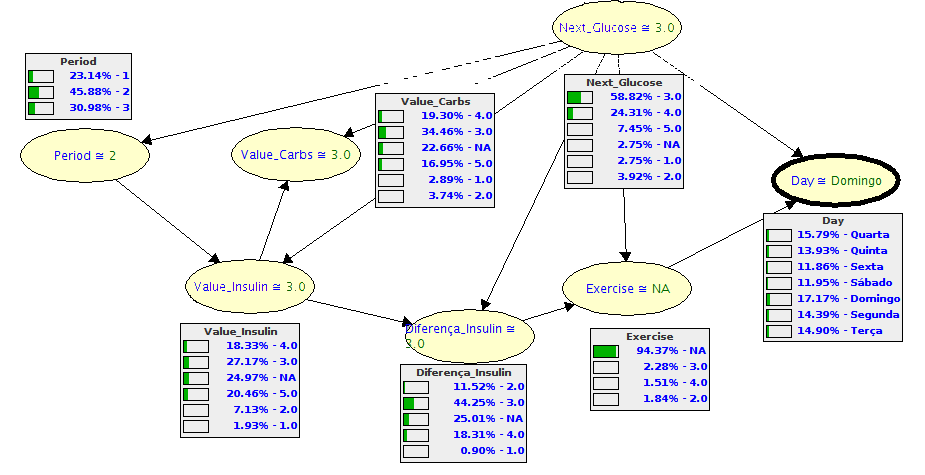
\includegraphics[height=65mm, width=130mm]{/home/tiago/Tese/Tese/Databases/CSV/Data/ImagensTese/Utilizador1/Sam.png}
\caption{Glicemia por horas do utilizador 5}
\end{figure}

É possível ver as tabelas de probabilidade para cada variável, sendo que cada nó tem por predefinição o valor mais frequente, como por exemplo, ``Next\textunderscore Glucose=3''. Note-se que os valores NA correspondem a registos que não usaram essas variáveis, isso é, um utilizador pode registar uma glicemia e não registar insulina ou hidratos d carbono. Estas tabelas também permitem perceber a distribuição de algumas variáveis: por exemplo, é possível verificar que, neste caso, os dias têm probabilidades muito parecidas, o que significa que têm um número parecido de registos. No entanto, tal como já mencionado, o objetivo nesta parte é tentar perceber de que forma estas variáveis afetam o valor da glicemia e também ver se estas alterações estão em concordância com as regras mostradas na secção anterior ou até ver se novos padrões surgem. Vamos, por isso, mostrar a rede \textit{bayesiana} para cada utilizador. 

\textbf{Utilizador 1}

Para este utilizador, a tabela de probabilidades inicial é mostrada na figura

\begin{figure}[H]
\centering
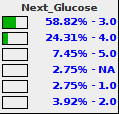
\includegraphics{/home/tiago/Tese/Tese/Databases/CSV/Data/ImagensTese/Utilizador1/Probs.png}
\caption{Glicemia por horas do utilizador 5}
\end{figure}

uma das regras geradas mostrava que, às quartas-feiras à tarde e quando o utilizador ingere hidratos de carbono em valores elevados, a glicemia tomava valores elevados. Ao selecionar, então, no SamIAm, esses três parâmetros com os valores definidos na regra, verifica-se que a probabilidade de ``Next\textunderscore Value=4'' sobe para 62.68\%.

Por outro lado, se colocarmos as variáveis de acordo com a regra para hipoglicemia neste utilizador, verificamos que a probabilidade de ``Next\textunderscore Glucose=2'' sobe para 34.74\%.

No entanto, é possível descobrir outros padrões: por exemplo, se selecionarmos apenas o dia ``Domingo'' verificamos que a probabilidade de uma hiperglicemia, ou seja um valor de glicemia 5, sobe para 18.67\%. 

Na figura seguinte pode-se ver quais os parâmetros que provocam uma probabilidade máxima de uma hiperglicemia.

\begin{figure}[H]
\centering
\includegraphics[height=65mm, width=130mm]{/home/tiago/Tese/Tese/Databases/CSV/Data/ImagensTese/Utilizador1/Hiper.png}
\caption{Glicemia por horas do utilizador 5}
\end{figure}

Ou seja, uma nova regra é descoberta: ao Domingo de manhã, quando o utilizador ingere uma quantidade grande de hidratos de carbono, tem maior probabilidade de ter uma hiperglicemia. 

\textbf{Utilizador 2}


A rede para o utilizador 2 é mostrada na figura seguinte

\begin{figure}[H]
\centering
\includegraphics[height=65mm, width=130mm]{/home/tiago/Tese/Tese/Databases/CSV/Data/ImagensTese/Utilizador2/Rede.png}
\caption{Glicemia por horas do utilizador 5}
\end{figure}

que, como se verifica, é ligeiramente diferente da rede gerada para o utilizador 1. Uma vez mais, é interessante ver quais os valores dos vários parâmetros que maximizam o valor de glicemia. 

\begin{figure}[H]
\centering
\includegraphics[height=65mm, width=130mm]{/home/tiago/Tese/Tese/Databases/CSV/Data/ImagensTese/Utilizador2/Hiper.png}
\caption{Glicemia por horas do utilizador 5}
\end{figure}

Como se pode observar, a probabilidade de hiperglicemia aumenta bastante aos sábados à tarde, quando o utilizador toma menos insulina que a recomendada. Esta regra não foi gerada pelo algoritmo \textit{apriori}, possivelmente por ter um valor de suporte abaixo do mínimo definido, mas ainda assim é uma regra interessante e que mostra uma utilidade desta análise. É interessante saber quais as condições em que o risco de hiperglicemia é maior, tendo em conta os dados já registados. 

\textbf{Utilizador 3}

A rede criada para o utilizador 3 está representada na figura

\begin{figure}[H]
\centering
\includegraphics[height=65mm, width=130mm]{/home/tiago/Tese/Tese/Databases/CSV/Data/ImagensTese/Utilizador3/Rede.png}
\caption{Glicemia por horas do utilizador 5}
\end{figure}

que é diferente das redes dos utilizadores anteriores, principalmente pelo facto de este utilizador não ter qualquer registo de exercício, pelo que essa variável não foi tida em conta.

\begin{figure}[H]
\centering
\includegraphics[height=65mm, width=130mm]{/home/tiago/Tese/Tese/Databases/CSV/Data/ImagensTese/Utilizador3/Hiper.png}
\caption{Glicemia por horas do utilizador 5}
\end{figure}

Como se pode ver na figura anterior, este utilizador tem uma probabilidade enorme de ter hiperglicemia à terça-feira à tarde, especialmente se tomar menos insulina que a calculada.  
\chapter{Conclusões}\label{chap:conc}

Ao longo desta dissertação fomos enfatizando duas coisas acerca da diabetes: é uma doença sem cura e, com tratamento adequado, os doentes diabéticos podem levar uma vida normal. Vimos também que não há um tratamento generalizado e que cada doente tem de ter um tratamento personalizado. Assim sendo, propusemos fazer diversos tipos de análise para um conjunto de utilizadores. Estas análises foram personalizadas para cada utilizador para tentar perceber que tipo de comportamentos é que os doentes diabéticos têm que provocam alterações na glicemia. Esta análise permitiu perceber que, de facto, diferentes utilizadores têm diferentes rotinas e hábitos e, portanto, incorrem em diferentes padrões. Na parte de regras de associação foi possível perceber que diferentes utilizadores tinham diferentes regras. Embora as regras possam ser do mesmo tipo, a parte importante é que são diferentes, evidenciando, uma vez mais, a importância de um tratamento individualizado. Também na parte das redes \textit{bayesianas} foi possível perceber esta necessidade: para cada utilizador foi gerada uma rede diferente e as variáveis relacionavam-se de maneira diferente em cada uma das redes. 
Foi ainda possível concluir a viabilidade do uso de \textit{data mining} em registos de doentes diabéticos: conseguimos gerar um número aceitável de regras diferentes com uma amostra de utilizadores pequena, o que faz prever que, para um conjunto bastante maior de dados, vão ser descobertos ainda outros tipos de padrões e portanto, auementar a variedade de regras. 



\section{Trabalho Futuro}\label{sec:trab}






%% appendix
\appendix
%% \include{app1}

%% references
%\renewcommand{\bibname}{Referências}
\cleardoublepage
\phantomsection
\addcontentsline{toc}{chapter}{\bibname}
\bibliographystyle{plainnaturlAuthor} % use plainnaturlAppear to order references by appearance 
% usually it is by author on thesis, to ease Author lookup
%\nocite{*}  % Include all entries in references.bib, not just the ones cited.
\bibliography{refs} %changed the env to make it a numbered chapter


%%%%%%%%%%%%%%%%%%%%%%%%%%%%%%%%%%%%%%%%%%%%%%%%%%
%%  Acronyms
%%%%%%%%%%%%%%%%%%%%%%%%%%%%%%%%%%%%%%%%%%%%%%%%%%
%\twocolumn

%%%%%%%%%%%%%%%%%%%%%%%%%
\chapter{Acrónimos}
%%%%%%%%%%%%%%%%%%%%%%%%%
\begin{multicols}{2}
\setlength{\columnseprule}{0.5pt}
\makeatletter
\@mkboth{\MakeUppercase Acrónimos}{\MakeUppercase Acrónimos}
\columnsep 35\p@
\makeatother
\begin{acronym}[HTTP] % o maior acrónimo
%------ Acronyms definitions
% http://www.ctan.org/tex-archive/macros/latex/contrib/acronym/
% Place the acronyms in alphabetical order as the acronyms chapter will not make automatically
\acro{IDF}{International Diabetes Federation}
\acro{OMS}{Organização Mundial da Saúde}
\acro{NA}{Not Available}
\acro{HbA1c}{Hemoglobina glicada}
\acro{WEKA}{Waikato Environment for Knowledge Analysis}
\acro{SamIAm}{Sensivity Analysis, Modeling, Inference And More}
\acro{CSV}{Comma-Separated Values}
\acro{CRAN}{Comprehensive R Archive Network}

\end{acronym}
\end{multicols}


%% bye
\end{document}
